\documentclass[prodmode,acmtois]{acmsmall}

\usepackage{amsfonts}
\usepackage{amssymb,amsmath}
\usepackage{xcolor}
\usepackage{times}
\usepackage[square,sort,numbers]{natbib}
\setlength{\bibsep}{0.0pt}
\usepackage{multirow}
\usepackage{booktabs}
\usepackage{xspace}
\usepackage{url}
\usepackage{enumerate}
\usepackage[bookmarksnumbered=true,bookmarksopenlevel=4,bookmarksopen=true]{hyperref} 
\usepackage{xcolor}
\definecolor{dark-red}{rgb}{1,0.15,0.15}
\definecolor{dark-blue}{rgb}{0.15,0.15,1}

\hypersetup{
 colorlinks   = true, %Colours links instead of ugly boxes
 urlcolor     = dark-red, %blue Colour for external hyperlinks
 linkcolor    = dark-red, % blueColour of internal links
 citecolor   = dark-blue, %green, %red %Colour of citations
}

\newcommand{\hh}{{\tt H}\xspace}
\newcommand{\rr}{{\tt R}\xspace}
\newcommand{\mm}{{\tt M}\xspace}
\newcommand{\nn}{{\tt N}\xspace}
\newcommand{\nkn}{{\tt N$_k$}\xspace}
\newcommand{\hkh}{{\tt H$_k$}\xspace}

\usepackage{pifont}% http://ctan.org/pkg/pifont
\newcommand{\cmark}{\ding{51}}%
\newcommand{\xmark}{\ding{55}}%
\usepackage{xcolor}
\usepackage{xargs}  
\usepackage[textsize=small]{todonotes}
%\newcommand{\sm}{\todo[author=\textbf{SM}, color=yellow,inline]}
\newcommandx{\ssm}[2][1=]{\todo[fancyline,author=\textbf{SM},linecolor=yellow,backgroundcolor=yellow,bordercolor=black,#1]{#2}}
%\newcommand{\aht}{\todo[author=\textbf{AHT}, color=green,inline]}
%\newcommand{\fs}{\todo[author=\textbf{FS}, color=cyan,inline]}

%\newcommand{\todo}[1]{\textcolor{red}{[{\bf #1}]}}
\newcommand{\sm}[1]{\textcolor{blue}{[{\bf SM: #1}]}}
\newcommand{\aht}[1]{\textcolor{green}{[{\bf AHT: #1}]}}
\newcommand{\fs}[1]{\textcolor{cyan}{[{\bf FS: #1}]}}
\newcommand{\ehm}[1]{\textcolor{orange}{[{\bf EHM: #1}]}}

%\newcommand{\myparagraph}[1]{\vspace{0.5\baselineskip}\noindent{\textbf{#1}}~}
\newcommand{\defineterm}[1]{\emph{#1}}


%% Avoid floats going to pages / columns by themselves
\renewcommand{\dbltopfraction}{0.9}  % fit big float above 2-col. text
\renewcommand{\textfraction}{0.07}  % allow minimal text w. figs
        %   Parameters for FLOAT pages (not text pages):
\renewcommand{\floatpagefraction}{0.7}  % require fuller float pages
          % N.B.: floatpagefraction MUST be less than topfraction !!
\renewcommand{\dblfloatpagefraction}{0.7} % require fuller float pages


 %\acmVolume{V}
 %\acmNumber{N}
 %\acmArticle{A}
 %\acmYear{YYYY}
 %\acmMonth{0}
\markboth{}{}

\title{On The Benefits of Magnitude Estimation Relevance Assessments
  for Information Retrieval Evaluation}

\title{Crowdsourcing Relevance Magnitudes for Information Retrieval
  Evaluation: On Using Magnitude Estimation to Gather Relevance
  Assessments by Means of Crowdsourcing}

\title{On Crowdsourcing Relevance Magnitudes for Information Retrieval
  Evaluation}

\author{
EDDY MADDALENA
\affil{University of Udine, Italy}
STEFANO MIZZARO
\affil{University of Udine, Italy}
FALK SCHOLER
\affil{RMIT University, Australia}
ANDREW TURPIN
\affil{University of Melbourne, Australia}
}

\begin{document}

\begin{bottomstuff}
Author's addresses: Eddy Maddalena, University of Udine, Udine 33100,
Italy, eddy.maddalena@uniud.it; 
Stefano Mizzaro, University of Udine, Udine 33100, Italy,
mizzaro@uniud.it; 
Falk Scholer. RMIT University, Melbourne, Victoria 3001, Australia,
falk.scholer@rmit.edu.au; 
Andrew Turpin, University of Melbourne, Melbourne, Victoria 3010,
Australia, aturpin@unimelb.edu.au. This paper is a revised and
extended version of \citet{ME-SIGIR15}.
\end{bottomstuff}




\input{0_abstract.tex}


\category{H.3.4}{Information Storage and Retrieval}{Systems and
  software}[performance evaluation] 
\terms{Measurement, performance, experimentation}
\keywords{Magnitude estimation, evaluation, relevance assessments,
  relevance} 

\acmformat{...}
\maketitle
% \sm{I think there are good reasons to add ``crowdsourcing'' to the title: the comment analysis is rather related to CS, and it may make sense to add a new CS-related RQ}
 

\section{Introduction}
\label{sec-intro}

Relevance is an important concept in information retrieval (IR), and
relevance judgments form the backbone of test collections, the most widely-used
approach
for the evaluation of IR system effectiveness.
Document relevance judgments are typically made using ordinal scales,
historically at a binary level, and more recently with multiple
levels~\citep{VooHar05}.
However, despite its importance, operationalizing relevance for
the evaluation of IR systems remains a 
complicated issue; for example,
when using an ordinal scale 
 it is unclear how many relevance categories should be
chosen~\cite{TanSha99}. 

Magnitude estimation is a psychophysical technique for measuring the
sensation of a stimulus.
Observers  assign numbers to a series of stimuli, such
that the numbers reflect the perceived difference in intensity of each
item.
The outcome is a ratio scale of the subjective perception of the
stimulus; if a magnitude of 50 is assigned to one stimulus, and 10 to
another, then it can be concluded that the two items are perceived in a
5:1 ratio of sensation~\cite{moskowitz:1977}.
While initially developed for the measurement of the sensation of
physical stimuli such as the intensity of a light source, magnitude
estimation has been successfully applied to the measurement of
non-physical stimuli including the usability of
interfaces~\cite{McG03}.

Being able to derive ratio scales of subjective perceptions of the
intensity of stimuli, magnitude estimation may be a useful tool for
measuring and better understanding document relevance judgments.
The application of magnitude estimation in the IR field has been
limited to the consideration of the relevance of carefully curated
abstracts returned from bibliographic databases~\citep{Eis88}, and our
own small-scale pilot study~\cite{SchMad14,MadMiz15}.
While suggestive, these studies have been limited in terms of
demonstrating the broader utility of the approach, or its direct
application to IR evaluation.
In this work, we investigate the larger-scale application of magnitude
estimation to document relevance scaling, reporting on a user study
over 18 TREC topics and obtaining judgments for 4,269 documents.
This is also the first work to consider the direct application of
magnitude estimation to the evaluation of IR systems, and to rely on
crowdsourcing workers to gather a large amount of magnitude estimation
relevance assessments.
Specifically, we consider four research questions.

\begin{enumerate}[RQ1.]
\itemsep 0em

\item \label{item:rq1} Is the magnitude estimation technique suitable
  for gathering document-level relevance judgments, and are the
  resulting relevance scales reasonable with respect to our current
  knowledge of relevance judgments?

\item \label{item:rq4} 
  Is crowdsourcing a viable method to gather robust magnitude
  estimation values?
  Crowdsourcing might exacerbate some of the
  potential complications of using magnitude estimation, such as the
  subjective scale used by each judge, or the difficulty in using a
  ratio scale without proper training.     
  Do the workers agree with
  previous judgments, and are 
  redundant workers required to obtain
  agreement with previous judging methods? 

\item \label{item:rq2} How does IR system evaluation change when ratio
  scale magnitude estimation relevance judgments are used to calibrate
  the gain levels of the widely-used nDCG and ERR evaluation metrics,
  compared to using arbitrarily set gain values for a pre-chosen
  number of ordinal levels?

\item \label{item:rq3} Can magnitude estimation relevance scores
  provide additional insight into user perceptions of relevance, into
  actual gain values, and into individual gain profiles?  

\end{enumerate}

We also investigate the qualitative comments that users of the magnitude
estimation relevance judging approach were required to make to justify
their scores, and present an analysis of the relationship between
comments, scores and source documents.

In the next section, background material and related work are
presented.
Details of our user study and experimental methodology are provided in
Section~\ref{sec-methods}, and the first descriptive results are
presented in Section~\ref{sec:descr-stat}.
The full analysis and discussion of our results, corresponding to the
four research questions, are detailed in Sections~\ref{sec-rq1}
to~\ref{sec-rq3}.
% Section~\ref{sec:comment-analysis} details the analysis of the comments that
% judges made to justify their magnitude estimation scores.
Our conclusions and directions for future work are included in the
final section of the paper.


% Local Variables:
% TeX-master: "ME-TOIS.tex"
% End:


\section{Background}
\label{sec-background}

\subsection{Relevance} 
%\myparagraph{Relevance:}
Relevance is an important concept in information science and
information retrieval~\cite{Sar07}.
IR system effectiveness is most often measured with reference to a test
collection, consisting of a set of search topics, a static set of
documents over which to search, and human-generated assessments that
indicate, for an answer document returned by a search system in
response to a topic, whether the document is relevant~\citep{VooHar05}.
Typically, these assessments are made based on ``topical'' relevance,
that is, a judgment of whether the document contains any information
that is ``about'' the material that the search topic is asking for.
Other aspects of relevance, such as novelty or contextual factors, are
not considered~\cite{Sar07}.
Based on the relevance judgments, each ranked answer list returned by
a system is aggregated into a number that reflects the system's
performance, using a chosen effectiveness metric.
The metrics themselves instantiate either implicit or explicit assumptions
about searcher behavior, for example that a relevant document that is
returned by a system lower down a ranked list is of less value
than if the same document had been returned earlier.

Historically, relevance judgments were often made using a 
\emph{binary} scale, where a document is classed as either being
relevant to the search topic or not, and many effectiveness metrics use
this notion of relevance, including 
\emph{precision}, \emph{recall}, 
\emph{mean average precision} (MAP), and \emph{precision at a specified cutoff}~\cite{VooHar05}.
More recently, based on the observation that searchers can generally
distinguish between more than two levels of relevance, evaluation
metrics that incorporate \emph{multi-level} relevance have been
proposed~\cite{JarKek02}.
Here, relevance is typically measured on an ordinal scale; metrics that
include this more fine-grained notion of relevance include 
\emph{normalized discounted cumulative gain} (nDCG)~\cite{JarKek02},
\emph{expected reciprocal rank} (ERR)~\cite{ChaMet09}, and the
\emph{Q-measure}~\cite{Sakai07}.
Some examples of previous choices for the number of levels in ordinal
relevance scales include 3 (TREC Terabyte Track~\cite{ClaCra04}), 4
(TREC newswire re-assessments by~\citet{Sormunen:2002}), and 6 (TREC
Web Track~\cite{ColBen14}).
\citet{TanSha99} studied the self-reported confidence of psychology
students when assessing the relevance of bibliographic records on
ordinal scales from 2 to 11 levels, and observed that for this specific
task, confidence is maximized with a 7-point scale.
However, the issue is far from settled: in a broader survey of the optimal number of levels in an ordinal
response scale, \citet{Cox80} concludes that there is no single number
of response alternatives that is appropriate for all situations.

\subsection{Magnitude Estimation} 

%\myparagraph{Magnitude estimation:}
Magnitude estimation (ME) is a psychophysical technique for the construction
of measurement scales for the intensity of sensations.
An observer is asked to assign numbers to a series of presented
stimuli.
The first number can be any value that seems appropriate, with
successive numbers then being assigned so that their relative
differences reflect the observer's subjective perceptions of
differences in stimulus intensity~\citep{EhrEhr99}.
A key advantage of using magnitude estimation is that the responses are
on a ratio scale of measurement~\citep{Ges97}, meaning that all mathematical operations
may be applied to such data, and parametric statistical analysis
can be carried out.
In contrast, for ordinal (or ranked category) scales certain operations
are not defined; for example, the median can be used as a measure of
central tendency for ordinal data, but the mean is not meaningful since
the distance between the ranked categories is not defined~\citep{She07}.

Proposed by Stanley Stevens in the 1950s, magnitude estimation
has a long history, and is the most widely-used psychophysical
ratio scaling technique~\cite{Ges97}.
Initially developed to measure perceptions of physical stimuli, such as
the brightness of a light or the loudness of a sound, magnitude
estimation has also been successfully applied to a wide range of
non-physical stimuli in the social sciences (including occupational
preferences, political attitudes, the pleasantness of odors, and the
appropriateness of punishments for crimes~\citep{Ste66}), in medical
applications (such as levels of pain, severity of mental disorders, and
emotional stress from life events~\citep{Ges97}), in user experience
research (for example, as a measure of usability in HCI~\citep{McG03},
and for health-care applications~\citep{Joh10}), and in linguistics
(including judging the grammaticality of sentences~\citep{BarRob96}).

In information retrieval research, 
\citet{Eis88} investigated magnitude estimation in the context of
judging the relevance of document citations from a library database
(including fields such as author, title, keywords and abstract), and
concluded that participants are able to effectively use magnitude
estimation in such a scenario.
A related technique was used by 
\citet{SpiGre01}, where
participants in a user study were required to fill in a worksheet with
information about the relevance of resources that were retrieved from a
library database for personal research projects; this included
indicating the level of relevance on a 4-level ordinal scale, providing
feedback about other levels of relevance such as utility and
motivation, and marking the level of relevance on a 77mm line.
The line was then decoded into numbers at a 1mm resolution
so was in effect a 78-level ordinal scale.

To the best of our knowledge, the only previous investigation of
magnitude estimation for document-level relevance judging in the
context of IR evaluation was our own small pilot study~\cite{SchMad14,MadMiz15}.
That study indicated that 
magnitude estimation could be useful for
measuring document-level relevance, but used only 
3 information need statements and 33 documents.
In this paper we carry out a much larger-scale study, across 18 TREC
topics and 4269 documents.
Unlike previous studies, 
our work also explores the application of this scaling approach to the
direct calibration of effectiveness metrics for IR system evaluation,
and the relationship between the magnitude relevance space and the
concept of gain.

\textcolor{red}{
This paper is based on a preliminary version published at 
SIGIR 2015~\cite{ME-SIGIR15}, but adds: RQ2; 
related background on crowdsourcing;
more information on the score distributions in Section~\ref{sec:descr-stat}, including
Figures~\ref{fig:ME-raw-scores} and~\ref{fig:ME-norm-scores} and their discussion;
a new Section~\ref{sec:cs} including Figure~\ref{fig:judgeVariability} and 
recomputation of Figure~\ref{fig:workersQuality};
new material in Section~\ref{sec:rq2}, including recomputation of 
Figures~\ref{fig:runs-rerank-median3best} and~\ref{fig:runs-rerank-median3best-fake}; 
a revised second half of Section~\ref{sec-rq3}; 
an Appendix giving exact participant instructions; and
additional references.
}


\subsection{Crowdsourcing}
\label{sec:crowdsourcing}

The third ingredient of our work is crowdsourcing. 
namely the outsourcing of a task usually performed by experts to a
crowd by means of an open call. 
Although criticized by some \cite{keen2008}, crowdsourcing has been
shown to be effective for several tasks, at least under some
conditions, and
% blog posts? 
% Iperiotis?,
it has been (and still is) much used as a method to collect relevance
judgments. 

For example \citet{Alonso:2012} compared relevance judgments gathered
by the crowd vs.\ more experienced TREC assessors, finding comparable
accuracy. 
Others have attempted to measure relevance in various ways, including
graded judgments \cite{mccreadie:2011}, preference-based judgments
\cite{Anderton2012}, and multidimensional ones \cite{Zhang2014}.
Collecting relevance labels through crowdsourcing has also been used
in practice, for example in the TREC blog track \cite{mccreadie:2011},
or in the judgment task of the TREC Crowdsourcing Track
\cite{Smucker2014}. 
Still in the IR field, it has been shown that crowdsourcing can be
effective not only to collect relevance judgments, but also for more
complex tasks \cite{Zuccon:2013}.


Of course, quality is an issue: workers might be too inexperienced for
some tasks, or even behave maliciously to finish the task without any
accuracy, perhaps even in a random way, just to gain money. 
Several papers address this problem.
For example, \citet{Clough2013} show that even if workers disagree,
system rankings might not change. 
\citet{Kazai2013} study how several factors (e.g., pay, effort, worker
qualifications, motivations, and interest) can affect the quality of
the relevance judgments collected.

Appropriate aggregation methods can be used as countermeasures to low
quality work. 
\citet{Hosseini:2012} and \citet{Jung2011} compare the classical
aggregation method of majority voting with more sophisticated
approaches that take into account a worker's expertise (based on
expectation maximization and outlier detection, respectively), finding
the latter to be more effective. 


In this work, we use crowdsourcing to gather magnitude estimation
relevance assessments at scale.
Apart from our own pilot studies \citep{SchMad14,MadMiz15} we
are not aware of any studies that uses crowdsourcing to gather magnitudes,
let alone using crowdsourcing to gather relevance judgments expressed
by magnitude estimation.
Since magnitude estimation is a process that is unlikely to be familiar
to the average crowd worker, analyzing the suitability of the crowd for
completing such tasks is novel.

% Local Variables:
% TeX-master: "ME-TOIS.tex"
% End:



\section{Experimental Methodology}
\label{sec-methods}

In this section we describe the details of the experiments that were
carried out to crowdsource
%gather
the required relevance judgments using magnitude estimation.

\subsection{Topics and Documents}

Document-level relevance assessments have traditionally been made using
binary or multi-level ordinal scales.
To compare magnitude estimation judgments to these approaches, we
selected a set of search tasks and documents from the TREC-8 ad hoc
collection, which studies informational search over newswire documents.
The TREC-8 collection includes binary relevance judgments made by
NIST assessors~\cite{VooHar99}. Subsequently, \citet{Sormunen:2002} carried out a
re-judging exercise where a subset of topics and documents were judged
by a group of six Master's students of information studies, fluent in English although not native speakers,
on a 4-level ordinal relevance scale: \nn--not relevant (0);  
\mm--marginally relevant (1); \rr--relevant (2); \hh--highly relevant
(3).

The 18 \emph{search topics} used in our study were the subset of TREC-8 topics
which also have Sormunen ordinal judgments available. 
They are listed in the first column of Table~\ref{tab:descr-stat}.
The \emph{documents} for which we collected magnitude estimation
judgments were the set of the top-10 items returned by systems that
participated in TREC-8.  
This gives a total of 4,269 topic-document pairs, of
which 3881 have binary TREC relevance judgments available, and 805 
of which have Sormunen ordinal judgments available.
The number of documents for each topic is shown in 
Table~\ref{tab:descr-stat} (2nd column). 

\begin{table}[t]%
%   \centering
% %\begin{footnotesize}
% \begin{scriptsize}
\tbl{Topics, number of documents, number of units, \hkh, \nkn, number of back buttons
  usage, number of failures in the (c) and (d) checks, as detailed in
  the text.\label{tab:descr-stat}%
}{%
%  \begin{tabular}{@{}l @{ } r @{ } r  l@{ }l  @{ }  r@{ }r@{ }r  @{ } c@{  } r@{ }r@{ }r@{}}
  \begin{tabular}{l rr  ll rrrcrrr}
\toprule
    Topic&
\multicolumn{1}{l}{No.}  & 
\multicolumn{1}{l}{No.}  &   
\hkh &
\nkn & 
\multicolumn{3}{c}{Back} && 
\multicolumn{3}{c}{Fail}\\ 
    & 
\multicolumn{1}{l}{docs} & 
\multicolumn{1}{l}{units} &    
&  
& 
\multicolumn{1}{c}{$0$} & 
\multicolumn{1}{c}{$1$}& 
\multicolumn{1}{c}{$\ge 2$} && 
\multicolumn{1}{c}{$0$}& 
\multicolumn{1}{c}{$1$}& 
\multicolumn{1}{c}{$\ge2$}\\ 

% \multicolumn{1}{@{}l@{}}{No.}  & 
% \multicolumn{1}{@{}l@{}}{No.}  &   
% \hkh &
% \nkn & 
% \multicolumn{3}{c}{Back} && 
% \multicolumn{3}{c}{Fail}\\ 
%     & 
% \multicolumn{1}{@{}l@{}}{docs} & 
% \multicolumn{1}{@{}l@{}}{units} &    
% &  
% & 
% \multicolumn{1}{@{}c@{}}{$0$} & 
% \multicolumn{1}{@{}c@{}}{$1$}& 
% \multicolumn{1}{@{}c@{}}{$\ge 2$} && 
% \multicolumn{1}{@{}c@{}}{$0$}& 
% \multicolumn{1}{@{}c@{}}{$1$}& 
% \multicolumn{1}{@{}c@{}}{$\ge2$}\\ 

\midrule
402	& 278	& 460	& LA111689-0162	& FBIS3-10954       & 452 &  8 & 0 && 426 & 18 & 16\\
403	& 111	& 182	& LA092890-0067	& LA071290-0133     & 178 &  4 & 0 && 120 & 19 & 43\\
405	& 214	& 354	& LA061490-0072	& FBIS3-13680       & 347 &  6 & 1 && 322 & 20 & 12\\
407	& 212	& 350	& FT921-6003	& FR940407-2-00084  & 346 &  3 & 1 && 324 &  9 & 17\\
408	& 188	& 310	& FT923-6110	& LA062290-0070     & 306 &  4 & 0 && 266 & 16 & 28\\
410	& 212	& 350	& FBIS4-64577	& FBIS4-44440       & 346 &  4 & 0 && 326 & 10 & 14\\
415	& 179	& 295	& FBIS3-60025	& FBIS4-10862       & 289 &  4 & 2 && 255 & 23 & 17\\
416	& 174	& 287	& FBIS4-49091	& LA112590-0107     & 286 &  1 & 0 && 267 & 12 &  8\\
418	& 243	& 402	& LA102189-0167	& FT924-6324        & 394 &  8 & 0 && 372 & 15 & 15\\
420	& 164	& 270	& LA121590-0108	& LA112690-0001     & 266 &  4 & 0 && 256 &  4 & 10\\
421	& 342	& 567	& FT941-428	& LA073189-0033     & 554 & 11 & 2 && 537 & 16 & 14\\
427	& 195	& 322	& FT943-5736	& LA080590-0077     & 315 &  7 & 0 && 214 & 52 & 56\\
428	& 253	& 419	& FT943-9226	& FBIS3-20994       & 412 &  6 & 1 && 396 & 13 & 10\\
431	& 203	& 335	& FBIS3-46247	& FT944-5962        & 333 &  2 & 0 && 296 & 27 & 12\\
440	& 264	& 437	& FT942-3471	& LA020589-0074     & 427 & 10 & 0 && 397 & 19 & 21\\
442	& 408	& 677	& LA011390-0057	& FT923-4524        & 672 &  5 & 0 && 629 & 25 & 23\\
445 	& 210	& 347	& FT924-8156	& LA031989-0092     & 334 & 11 & 2 && 334 & 10 & 3 \\
448	& 419	& 695	& LA080190-0139	& FBIS3-16837       & 687 &  8 & 0 && 652 & 21 & 22\\
\addlinespace                                                              
Sum:	&4269	&7059	&		&	            &6944& 106 & 9 &&6389 &329 &341 \\ 
\multicolumn{2}{@{}l@{}}{Percentage:}&&  &                   &  98 &  2 & 0 &&  90 & 5  & 5 \\
\bottomrule
  \end{tabular}%
}%
%\end{scriptsize}
\end{table}


\subsection{User Study}

We carried out a user study through the CrowdFlower crowdsourcing
platform during December 2014 and January 2015.
The experimental
design was reviewed and approved by the RMIT University 
ethics
review board.
Participants were paid \$0.2 for each task \emph{unit}, defined as a group of
magnitude estimation judgments for 8 documents in relation to one
topic. 
The number of units for each topic is shown in
Table~\ref{tab:descr-stat} (3rd column). 

\subsubsection{Practice task}
\label{sec:practice-task}

%\myparagraph{Practice task:}
After agreeing to take part in the study, a participant was shown 
a first set of 
task
instructions, including a brief
introduction to the experiment and explanation of the
magnitude estimation process.
Since magnitude estimation may not be familiar to participants, they
were first asked to complete a practice task, making magnitude
estimations of three lines of different lengths, shown one at a time.
If they successfully completed this practice task (success was defined
as assigning magnitudes such that the numbers were in ascending order
when the lines were sorted from shortest to longest), participants were
able to move on to the main part of the experiment.
The full instructions shown to participants for the practice task are
included in Appendix A.

\subsubsection{Main task}
\label{sec:main-task}


%\myparagraph{Main task:} 
The main task of the experiment required
making magnitude estimations of the relevance of documents.
Participants were informed, by means of a second set of instructions,
that they would be shown an information need statement, and then a
sequence of eight documents that had been returned by a search system
in response to the information need statement, presented in an
arbitrary order, and that their task was to 
\emph{indicate how relevant these documents appear} in relation to the information need. 

For the main task, the title, description and narrative of a TREC topic
were first displayed at the top of the screen.
After reading the information need, participants had to respond to a
4-way multiple-choice question, to test their understanding of the
topic.
The test questions focused on the main information concepts presented
in the topic statements, and were intended to check that participants
were engaging with the task, and as a mechanism to remove spammers.
Participants who were unable to answer the test question correctly were
unable to continue with the task.

Next, participants were presented with eight documents, one at a time.
For each document, the participant was required to enter a magnitude estimation 
number in a text box displayed directly below the document, and 
a brief justification of why they
entered their number into a larger text field.
They were then able to proceed to the next document.
A back button was available in the interface, with participants being
advised that this should only be used if they wish to correct a mistake;
under 3\% of submitted jobs included use of this feature 
(details on the occurrences of clicks on the back button are shown in
Table~\ref{tab:descr-stat}, where the number of units with zero, one, or two
or more back button clicks are shown).

After entering responses for eight documents, the task was complete.
Participants were able to complete further tasks for other topics, up
to a maximum of 18 tasks, as they were not able to re-assess the same
topic.

\subsubsection{Magnitude estimation assignments}
\label{sec:magn-estim-assignm}

%\myparagraph{Magnitude estimation assignments:} 
Participants were instructed 
to assign ME scores as follows.
\emph{You may use any numbers that seem appropriate to you -- whole numbers,
fractions, or decimals.
However, you may not use negative numbers, or zero.
Don't worry about running out of numbers -- there will always be a
larger number than the largest you use, and a smaller number than the
smallest you use.
Try to judge each document in relation to the previous one.
For example, if the current document seems half as relevant as the
previous one, then assign a score that is half of your previously
assigned score.} 
While some applications of
magnitude estimation use a fixed modulus (specifying a particular number that
is to be assigned to the first stimulus that is presented), this has
been found to promote clustering of responses and the potential
over-representation of some numbers~\cite{moskowitz:1977}; we therefore
allowed participants to freely choose their own values.
The complete
instructions that were shown to participants for both the practice and
main tasks are included in Appendix A.

\subsubsection{Document ordering}
\label{sec:document-ordering}

% \myparagraph{Document ordering:} 
As explained above, each participant
task \emph{unit} required the judging of a set of eight documents for a particular search
topic statement.
The experiments used a randomized design, with documents presented in
random order, to avoid potential ordering effects and first sample
bias~\cite{moskowitz:1977}.
The document sets were constructed such that two of the documents in
each set were a known ordinal \hh and \nn document for the topic;
%
these documents %(referred to in the following as
(henceforth \hkh and \nkn) were the same for all 
the participants working on the same topic 
(the TREC document identifiers for each
topic are shown in Table~\ref{tab:descr-stat}).
This was to ensure that each participant saw at least one document from
the high and low ends of the relevance continuum.
Ensuring that stimuli of different intensity levels are included in a
task has been found to be important for the magnitude estimation
process~\cite{Ges97}, and also has an impact on the score normalization
process, described below.
Moreover, including the two \nkn and \hkh documents with ``known'' ordinal relevance
values enabled a further data collection quality control check: after
judging all eight documents, participants who had assigned magnitude
estimation scores for the \nkn document that were larger than for the
\hkh document were not able to complete the task.
In total, at least 10 ME scores were gathered for each topic-document
pair.

\subsubsection{Quality checks}
\label{sec:quality-checks}

% \myparagraph{Quality checks:} 
In total, four quality checks were included in the
data gathering phase of our experiments: 
%\vspace{-0.5em}
\begin{enumerate}[(a)]
%\itemsep 0em
\item a practice task requiring magnitude estimation of line lengths; 
\item a multiple-choice test question to check a participant's
understanding of the topic; 
\item a check that the magnitude estimations score for \hkh was greater than that
assigned to \nkn; and 
%\end{enumerate}
%\vspace{-0.5em}
%In addition, a time-based quality check was also used: 
%\vspace{-0.5em}
%\begin{enumerate}[(d)]
\item each participant had to spend at least 20 seconds on each of the
8 documents.
\end{enumerate}
%\vspace{-0.5em}
%
If any of (a) or (b) was unsuccessful, the participant could not
continue with the task.
They were allowed to restart from scratch, on a
different unit and therefore on a randomly selected topic, if willing
to do so; the same quality checks were applied again.
If checks (c) or (d) were unsuccessful, the participant received the
message ``\emph{Your job is not accurate enough.
You can revise your work to finish the task}'', and was allowed to use
the back button and revise their previously assigned scores if they
wished (the same two checks (c) and (d) were performed again in such a
case); however, participants were not made aware which documents or
scores were the ``offending'' responses.
Less than 10\% of units resulted in conditions (c) or (d) being
triggered (see details in Table~\ref{tab:descr-stat}, where the number
of eventually successful units with 0, 1, or two or more failed checks
are shown), and as already mentioned the back button was used in less
than 3\% of units.
Finally, there was a syntax check that the numeric scores input by the
participants were in the $(0,+\infty)$ range.
If any of the checks were not successfully completed, no data for that
unit was retained.
Based on these extensive quality checks, we did not carry out 
any further filtering once the data had been collected.



% Local Variables:
% TeX-master: "ME-TOIS.tex"
% End:


\section{General Results and Descriptive Statistics}
\label{sec:descr-stat}

% \sm{move here ``Crowd judging''?}

\subsection{Crowd Judging}
\label{sec:crowd-judging}

%\myparagraph{Crowd Judging:}
As detailed in Table~\ref{tab:descr-stat}, with 7,059 units comprised
of 8 documents each, we collected more than 50,000 judgments in total,
at a cost of around $\$1,700$ (CrowdFlower fees included).
This is in the order of magnitude of $\$0.4$ for each document, which
is broadly competitive when compared with the cost of TREC assessors
or other similar crowdsourcing initiatives; for example, according to
\citet[Footnote~2]{Alonso:2012}, gathering ordinal scale judgments
cost around $\$0.1$ per document.
However, the comparison is more favorable when considering that in our
experiments 10 redundant judgments per document are collected, and the
\nkn and \hkh documents receive multiple judgments, whereas in Alonso
and Mizzaro's work only 5 redundant judgments were collected, and
there was nothing similar to our \nkn vs. 
\hkh check.
We return to the cost issues in more detail in 
Section~\ref{sec:how-many-workers}, where the number of repeat
judgments that are required for stable ME estimates is investigated.  

In total, 1481 workers participated in our experiments. 
Since it was impossible for a worker to perform the task twice (or
more) for each topic, each worker could complete between 1
(around 30\% of the workers did so) and 18 (less than 1\% of the
workers) tasks.
As is usual in similar crowdsourcing experiments, the distribution
of the number of tasks for a worker resembles a power law, although
with only 18 tasks at maximum it is difficult to be precise on that.
Finally, workers tend to work in sessions: when they complete a topic they
either leave after that, or sometimes they complete a subsequent topic
straight away---they much more rarely leave and come back later to
do another.
% In Section~\ref{sec:comment-analysis} we consider the effect that this
% has on 
% the comments left by the workers.
% \fs{Check that this is actually included in the final version of
% Section~\ref{sec:comment-analysis}.}

\subsection{Score Distribution}
\label{sec:score-distribution}

\begin{figure}[t]
  \centering
  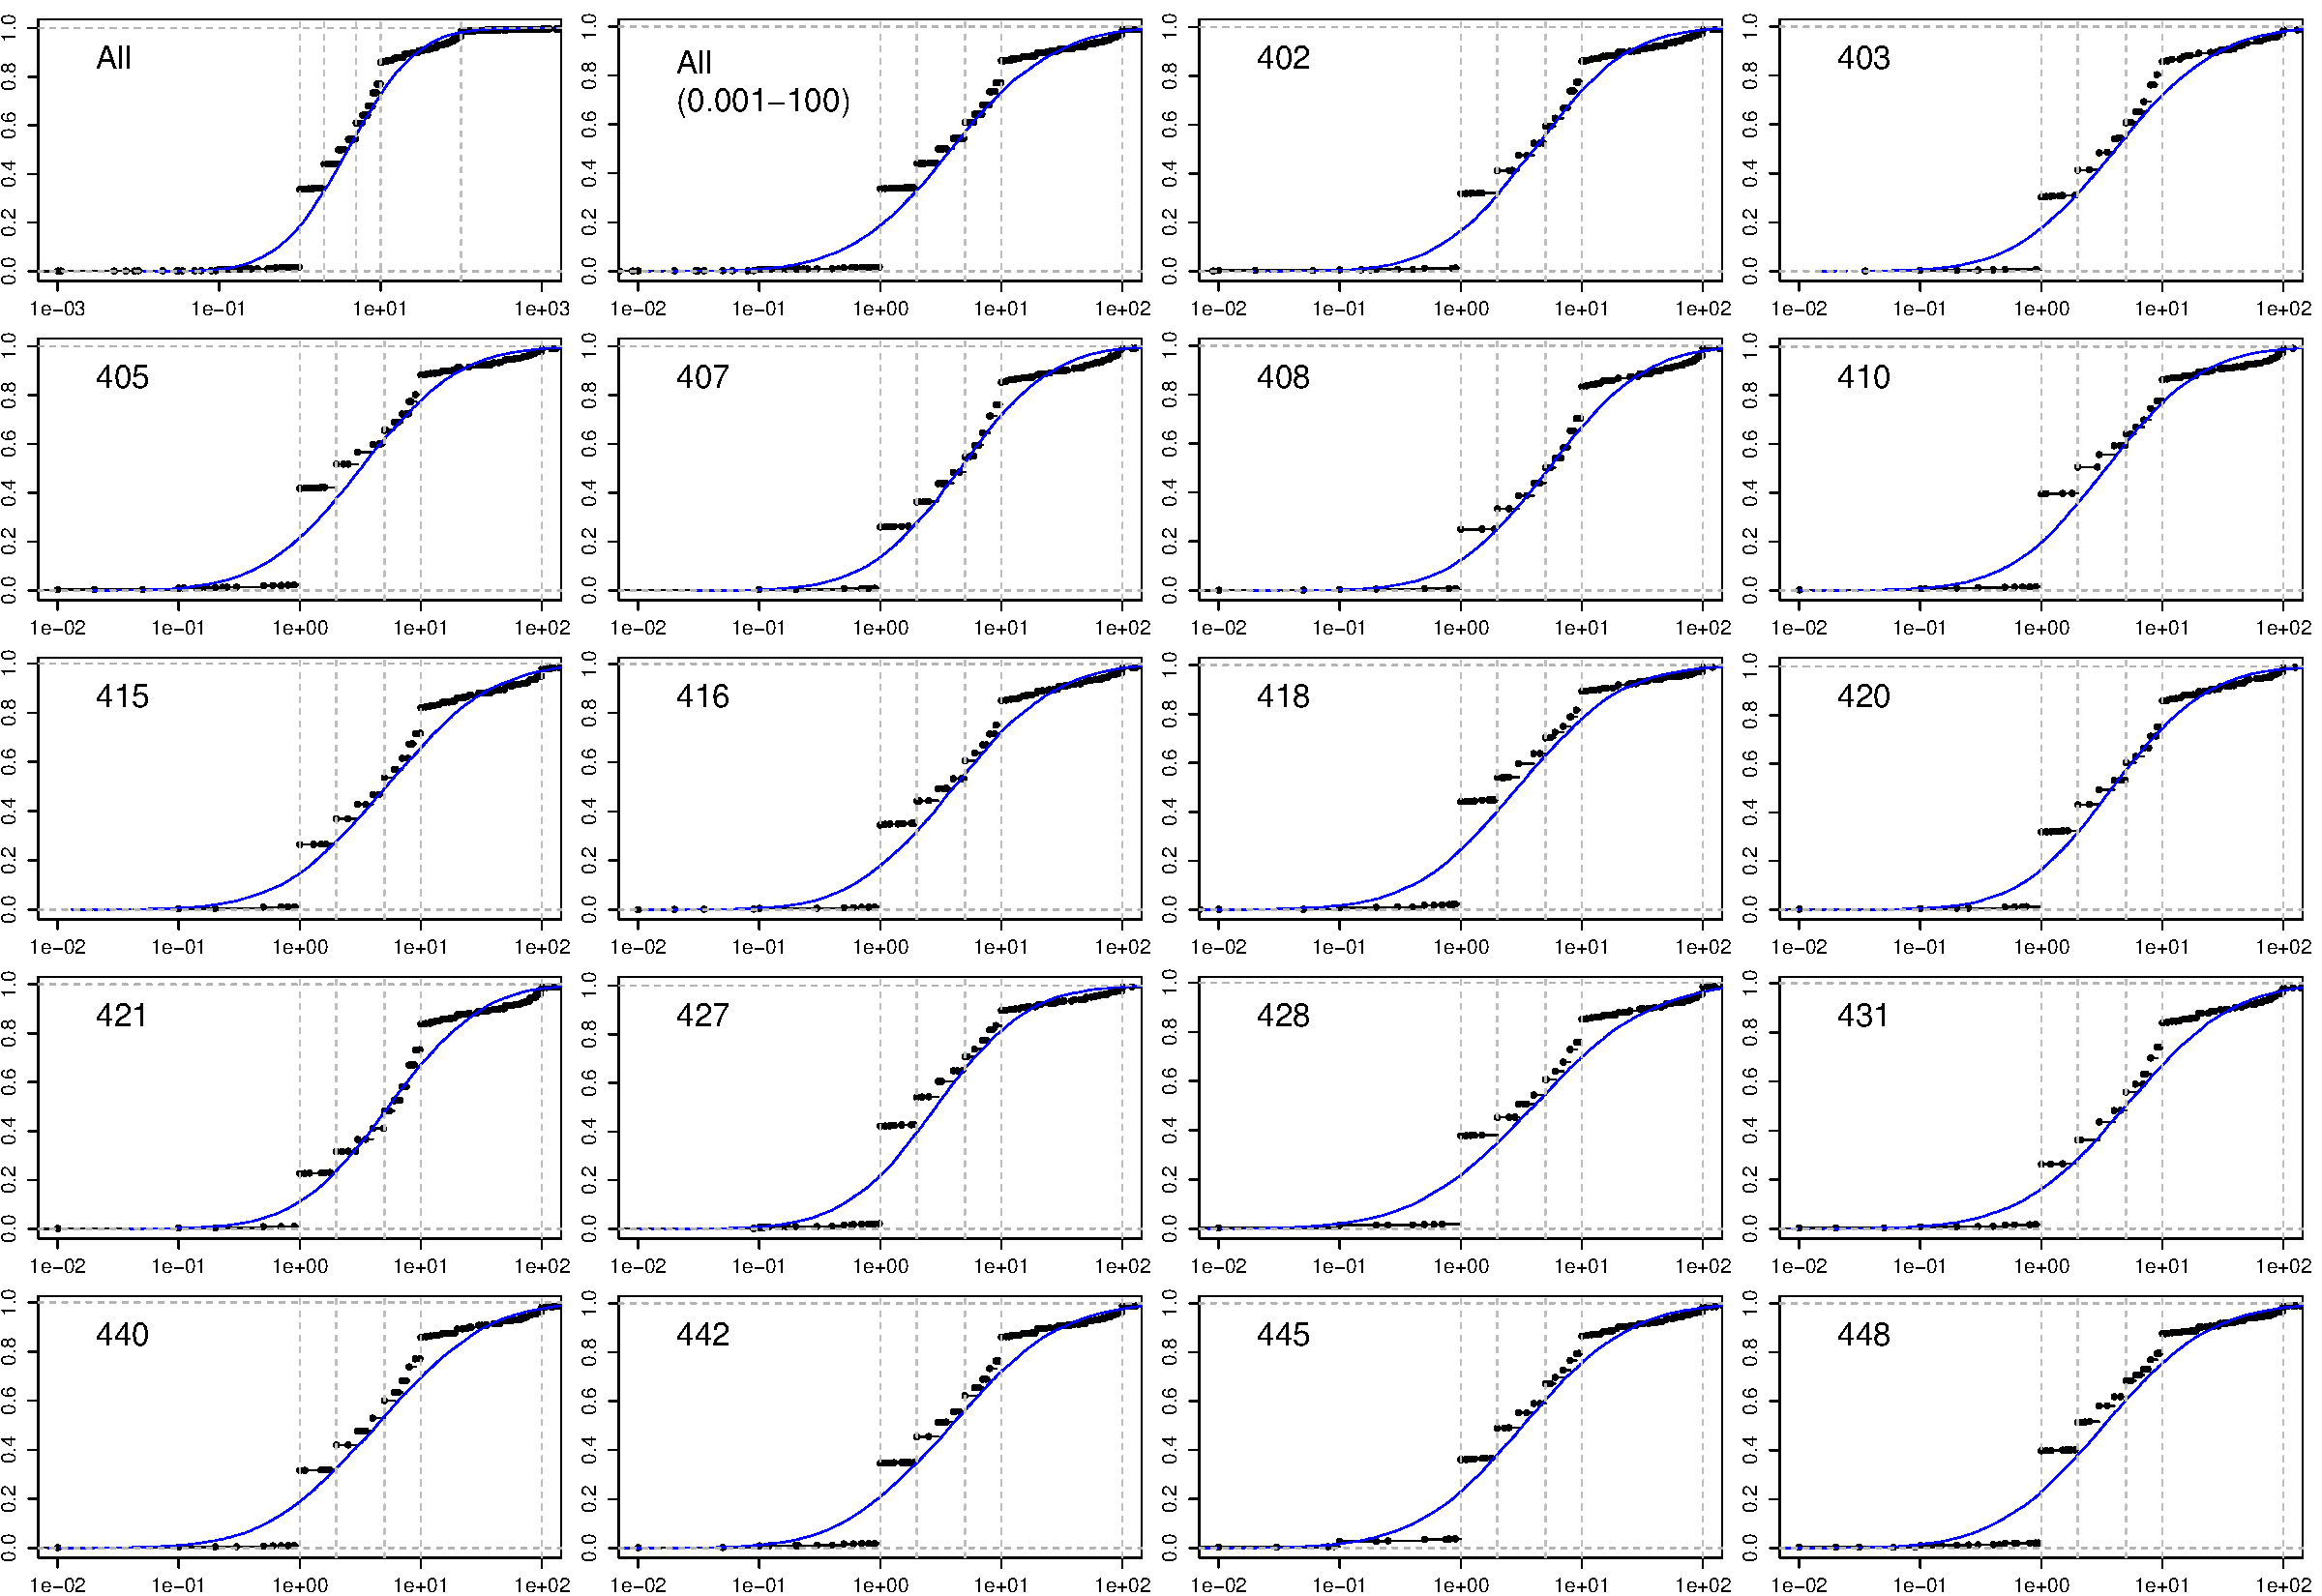
\includegraphics[width=\linewidth,page=1]{figs/MEscores.pdf}
  \caption{Cumulative distribution functions of raw ME scores for each topic 
(labelled in the top left of each panel) for all scores in the range
0.01 to 100. Black dots are gathered scores and the blue line in each panel is a 
fitted log-normal curve. The x axis is a log scale. 
Vertical dashed lines are at 1, 2, 5 and 10.}
  \label{fig:ME-raw-scores}
\end{figure}

Magnitude estimation scores should be approximately
log-normal~\citep{Mar74,moskowitz:1977}. 
%\sm{ks test on the logs does not indicate normality but...}
Figure~\ref{fig:ME-raw-scores} shows the situation for our data, 
plotting the Cumulative Distribution Functions (CDFs) of:
all the scores (top left), all the scores in the $0.001$-$100$ range
(which includes about 99.5\% of the scores), and the scores for each
topic. 
The continuous blue lines are fitted log-normal distributions with the
same mean and standard deviation of the corresponding data.  
From the figure it is clear that the log-normal distribution is a
reasonable approximation of the raw data. 
Differences are generally due to a \emph{round number tendency}
\cite{moskowitz:1977}: in general, people expressing magnitudes using
a numeric scale tend to use some specific values more than others, for
instance integer numbers and powers of ten. 
From the figure it can be seen that our workers tended to use
especially 1, 2, 5, and 10 (the values where ``steps'' can be seen on
the CDF curves --- see the gray vertical dashed lines on the charts),
and also quite a lot of 3, 4, 5, 6 7, 8, 9, 20, 30, 40, 50, 60, 70,
80, 90, and 100. 
The breakdowns on single topics show that topics do have an effect
(for instance, in topics 418 and 421 the scores up to~1 included
account for about 44\% and 23\% of the values respectively), although
the general trend is very similar, as is again demonstrated by the
fitted log-normal distributions.
Topic means ranged from 7.9 to 12.9, and topic standard deviations ranged
from 17.5 to 23.2.

% raw scores means
%      402       403      405       407       408       410       415 416 
%10.013831 10.014614 8.595449 11.392839 12.990020 10.409096 12.467627 10.079280 
%      418       420       421       427       428       431       440 442 
%8.069978 10.199124 12.662327  7.903648 11.308172 11.505793 10.237795 10.398175 
%      445       448 
%9.081898  9.197152 

% standard deviations of raw scores
%     402      403      405      407      408      410      415      416 
%19.20965 19.59646 17.96137 21.16121 23.24930 21.54687 22.91172 19.67080 
%     418      420      421      427      428      431      440      442 
%17.87859 19.53965 22.58363 17.53647 22.80461 21.33762 20.23102 21.00615 
%     445      448 
%18.92293 19.69537 

\subsection{Score Normalization and Aggregation} 
\label{sec:score-normalization}

Magnitude estimation is a highly flexible process, with observers being
free to assign any positive number, including fractions, as a rating of
the intensity of a presented stimulus.
The key requirement is that the ratio of the numbers should reflect the
ratio of the differences in perception between stimulus intensities.
As the stimuli are presented in a randomized order, and observers are
free to assign a number of their choice to the first presented item, it
is natural that different participants may make use of different parts
of the positive number space.
Magnitude estimation scores are therefore normalized, to adjust for
these differences.
Geometric averaging is the recommended approach for the normalization
of magnitude estimation scores~\cite{Ges97,McG03,moskowitz:1977}, and
was applied in our data analysis.
Recall that for a given search topic, participants made magnitude
estimation judgments for groups of eight documents (a unit).
To normalize the scores, first the log of each raw score, $s_i$, is
taken. Next, the arithmetic mean of these log scores is calculated for
each {\emph{unit}} of 8 documents, and for the {\emph{topic}} as a
whole. 
Each individual log score is then adjusted by the unit and topic means,
and the exponent is taken of the resulting quantity, giving the final
normalized score 
\begin{align}
  s'_i &= e^{\log(s_i) - \mu(\log(\mathnormal{unit})) + \mu
           (\log(\mathnormal{topic})) } \label{eq:1}
\end{align}
% To normalize the scores, first the log of each raw score, $s_i$, is
% taken.
% Next, the arithmetic mean of these log scores is calculated for each
% unit of 8 documents ($\mu_u$), and for the topic as a whole ($\mu$).
% Each individual log score is then adjusted by the unit and topic means,
% and the exponent is taken of the resulting quantity, giving the final
% normalized score 
% \begin{align}
% s'_i &= \exp(\log(s_i) - \mu_u + \mu ). \label{eq:1} 
% \end{align}
An alternative equivalent formalization is: 
\begin{align}
s'_i &= s_i \cdot \frac{\gamma}{\gamma_u}, 
\label{eq:2}
\end{align}
where $\gamma_u$ is the geometric mean for each unit and $\gamma$ is
the geometric mean for the topic as a whole.
The log transformation is theoretically motivated by the fact that
magnitude estimation scores of perceived stimulus intensities have been
found to be approximately log-normal, which was the case in our data as
shown in Section~\ref{sec:score-distribution}. Intuitively,
normalization by geometric averaging means that the raw magnitude
estimation scores are moved along the number line, both in terms of
location and spread, and the individual differences in scale are
nullified.
For example, as shown by both 
\citet{moskowitz:1977} and  
\citet{McG03}, 
if two judges assigned scores of \{1, 2, 3, 4\} and \{10, 20, 30, 40\}
to the same set of four items, respectively, then the normalized values
would be identical in the two cases, as can be easily verified by
applying either Equation~(\ref{eq:1}) or~(\ref{eq:2}).
Importantly, normalization through geometric averaging has the property
of preserving the ratios of the original scores, the essential feature
of the magnitude estimation process.
%\sm{So, in the example above, 2, 3, 4, 5 would be normalized into something different,  as the ratios are different.}
%
\begin{figure}[tp]
  \centering
  \includegraphics[width=\linewidth,page=2]{figs/MEscores.pdf}
  \caption{CDFs of normalized ME scores using the
    same style as Figure~\ref{fig:ME-raw-scores}.
  \label{fig:ME-norm-scores}}
\end{figure}

Other normalizations have been proposed, 
for example using the median or the arithmetic mean instead of the
geometric mean (especially when zero is an allowed score, so the
geometric mean cannot be used)~\citet{moskowitz:1977}.
Other approaches include carrying out an additional calibration task
that is aimed at understanding the differences in individual scales;
in our scenario, this might be implemented by exploiting the \nkn and
\hkh documents, or in a more implicit way by relying on the maximal
and minimal scores expressed by each worker.

Unless otherwise noted, all analysis reported in this paper uses
magnitude estimation scores normalized by geometric averaging.
Geometric averaging normalization is in principle adequate since, as
we have discussed, our scores are approximately log-normal and they do
not include zero. 
Figure~\ref{fig:ME-norm-scores} shows the distribution of scores after
normalization which are similar to 
Figure~\ref{fig:ME-raw-scores}.
It can be noted how the normalization has the effect of smoothing the
scores (the round number tendency disappears, since each score is moved by a
quantity which is different for each worker) and of making them even
more log-normal.
%\aht{Does the ks test show (log) normal for this one?}

%%%?\begin{figure}[tp]
%%%?  \centering
%%%?  \includegraphics[width=\linewidth]{figs/MEscores-boxplot.png}
%%%?  \caption{Normalized  ME scores (y log scale) per topic.
%%%?  \label{fig:ME-norm-scores-boxplot}}
%%%?\end{figure}
%%%?
%%%?The boxplots of the normalized ME scores are shown in
%%%?Figure~\ref{fig:ME-norm-scores-boxplot}: the topic differences are
%%%?more clear here, and \sm{statsig test? 
%%%?  topic difficulty blahblahblah??} 
%%%?\fs{I suggest that we leave this fig out. 
%%%?  The per-topic distributions are avaliable (although split by Sorm
%%%?  level) in the other fig (two figs on) anyway, and IMO it would be
%%%?  better to *not* mention ``topic difficulty'', except perhaps as
%%%?  future work, and then do it properly as future work.} 
%%%?\sm{I leave it by now but I rather agree. 
%%%?  Andrew?}

% \subsection{Score aggregation[.5pg]}
% \label{sec:score-aggregation}

The problem of aggregating several ME scores for the same item also
needs some attention. 
For each topic-document pair we collected at least 10 ME scores, by 10
different workers (many more for the \nkn and \hkh documents). 
In the following we will primarily use the \emph{median} of the normalized ME
scores for a topic-document pair, although again alternatives are available at this step,
such as using the arithmetic mean or
the geometric mean of obtained ME scores~\cite{moskowitz:1977}. 
We briefly examine the effect of 
different normalization and aggregating schemes
on our findings in Section~\ref{sec:judge-agreement}.

% Local Variables:
% TeX-master: "ME-TOIS.tex"
% End:

\section{Magnitude Estimation Relevance Judgments}
\label{sec-rq1}

Having obtained magnitude estimation scores for 4,269 topic-document
pairs, we analyze the user-perceived relevance to answer the first
research question RQ\ref{item:rq1}, whether the magnitude estimation
technique is suitable for gathering document level relevance
judgments, and whether the resulting relevance scales are reasonable
with respect to our current knowledge of relevance judgments.

% \subsection{Consistency of Magnitude Estimation and Ordinal Relevance}
% \label{sec:cons-magn-estim}

\begin{figure}[t]
  \centering
  \includegraphics[width=.7\linewidth,page=19]{figs/check_gross_ranks_med.pdf}
  \vspace{-0.5cm}
  \caption{ME score distribution by Sormunen and TREC levels.}
  \label{fig:ME-distribution}
\end{figure}


\begin{figure}[tp]
  \centering
  %\includegraphics[angle=90,height=.9\textheight,page=1]{figs/check_gross_ranks_med_all.pdf}
  \includegraphics[width=\linewidth,page=1]{figs/check_gross_ranks_med_all.pdf} %
  \caption{ME score distribution by Sormunen (U, N, M, R, H) and TREC (U, 0, 1) levels:
    breakdown for individual topics.
  \label{fig:ME-distribution-breakdown}
   }
\end{figure}

The distribution of the median normalized magnitude estimation scores
for each document are shown in Figure~\ref{fig:ME-distribution},
aggregated across all 18 topics, and split by Sormunen ordinal
relevance levels (left side of figure, levels are 
\nn, \mm, \rr, \hh, and {\tt U}, the group of documents that were not judged
by Sormunen), and by TREC binary levels (right side of figure, levels
are $0$, $1$, and {\tt U}, the documents that were not judged by TREC,
as not all participating runs were included in the judging pool).
Boxplots in this paper show the median as a solid black line; boxes
show the 25th to 75th percentile; whiskers show the range, up to 1.5
times the inter-quartile range; and outliers beyond this range are
shown as individual points.

There is a clear distinction between each of the four adjacent Sormunen
levels (two-tailed t-test, $p<0.002$), with the magnitude estimation
scores on average following the ordinal scale rank ordering.
The differences between the two TREC levels are also significant
($p<0.001$), with the magnitude estimation scores on average again
being aligned with the binary levels.
This is strong evidence for the overall validity of the magnitude
estimation approach.

Figure~\ref{fig:ME-distribution-breakdown} shows the magnitude
estimation score distributions for each of the 18 individual topics.
Although there is some variability across topics, overall the figure
confirms that the magnitude estimation scores are generally aligned
with ordinal categories even when considering individual topics: the
medians of the median magnitude estimation scores (the solid black
lines) generally follow the ordinal categories, for all categories and
for all topics (there are a small number of exceptions for some of the
Sormunen adjacent categories in topics 403, 405, 410, 420, 421, and
440; there are no exceptions for non-adjacent categories, nor for TREC
categories).
Since for each topic there could potentially be 3 exceptions for
adjacent categories, and 6 exceptions in general, plus one exception
for the two TREC categories, the 6 exceptions found are out of $3 * 18
+ 18 = 72$ possible cases when considering only adjacent categories, or
out of $6 * 18 + 18 = 126$ cases when considering also non-adjacent
categories.
Such a limited fraction of exceptions (in the $5\%$-$8\%$ range) is
further strong evidence for the validity of our approach, even at the
single topic level.

Regarding the set of documents that were not judged by Sormunen
(left-most boxes in Figure~\ref{fig:ME-distribution} and sub-plots in
Figure~\ref{fig:ME-distribution-breakdown}), based on the magnitude
estimation scores it can be inferred that the bulk of this class are
likely to be non-relevant; however there are also instances that occur
across the central parts of the marginal to highly relevant score
distributions. There were also a handful of documents unjudged by 
TREC that seemed to be rated highly by our judges.
While the overall distributions of
magnitude estimation scores are strongly consistent with the ordinal
and binary categories, there are also documents in each class 
where the ME scores 
fall into the central region of a different class.
We therefore next investigate judge agreement.


% \subsection{Judge Agreement}
% \label{sec:judge-agreement}


% Local Variables:
% TeX-master: "ME-TOIS.tex"
% End:

\section{Magnitude Estimation and Crowdsourcing}
\label{sec:cs}

We now turn to the second research question and 
investigate whether crowdsourcing is a valid methodology to gather magnitude
estimation scores. 
We have already touched upon several related issues: the quality
checks that we put in place in our experiment and that allowed us to
gather good quality data (Section~\ref{sec:quality-checks}); the
approximately log-normal distribution of our magnitude estimation
scores (Section~\ref{sec:score-distribution}); the normalization and
aggregation functions (Section~\ref{sec:score-normalization}); and the
overall agreement of the magnitude estimation scores with official
relevance judgments (Section~\ref{sec-rq1}). 
We now present more details, focusing on measuring judge
agreement, on analyzing disagreement with official judges, and on
discussing what happens when the number of collected judgments 
decreases.

%\fs{ We didn't record the ``rubbish'' workers, they were prevented
%  from carrying out the task, so we can't do an analysis of what
%  happens if they are kept in.
%  Let's keep this RQ for later in the paper, and in that place repeat
%  some of the analysis using the median of 5 and 3 (instaed of 10) ME
%  judgments?}
%
%\sm{I've left this note here but I'm not sure I understand it...}

\subsection{Judge Agreement and Quality}
 \label{sec:judge-agreement}
It is well-known that relevance is subjective, even when focusing on
``topical'' relevance as is typically done in evaluation campaigns such
as TREC, and that judges will therefore not perfectly agree.
We define and discuss two kinds of agreement:
\begin{itemize}
\item \emph{internal}: agreement within one group of workers judging the
  same topic-document pair; and 
\item \emph{external}: agreement with expert judges (TREC,
  Sormunen). 
\end{itemize}
  
\subsubsection{Internal Agreement}
\label{sec:internal-agreement}

In our data, there are
at least ten workers judging the same topic-document pair, and
the source of internal disagreement might be threefold:
(i) the arbitrary, personal scale used by a judge when expressing an ME
score; 
(ii) the subjective nature of relevance; and 
(iii) the often-feared low quality of work in crowdsourcing exercises.
The first has already been discussed and is removed by the geometric
average normalization process (Section~\ref{sec:score-normalization}).
The second is a feature that one might not want to remove from the
data: different judges can truly have different opinions on the
relevance of a document, whatever scale of measurement is used.
Usually IR evaluators assume that this variation is distilled into a single 
value (for example: mean, median or mode) 
that represents a population of users.
Of course, the third source is in need of particular attention: low
quality workers might express unreliable scores, and in general this
would lead to low internal agreement.

To examine internal agreement, we can investigate the spread of 
the 10 normalized scores collected for each topic-document pair.
Being on a ratio scale, an appropriate way of quantifying the upper
limit of the spread is
by the ratio between maximum and minimum $\max(s'_i) / \min(s'_i)$.  
Figure~\ref{fig:judgeVariability} 
shows the distribution of the ratio in our data.
Another measure of dispersion that can be used is the geometric
standard deviation (a version of standard deviation adapted for
geometric mean and log-normal distributions). 
The chart on the right of the figure shows that the geometric standard
deviation correlates quite well with the max/min ratio (Pearson's
correlation is $0.999$), and therefore is an almost equivalent
measure. 

\begin{figure}[tp]
  \centering
  \includegraphics[width=.9\linewidth,page=6]{figs/JudgeVariability.pdf}
%  \includegraphics[width=.29\linewidth,page=2]{figs/MaxMin-gsd_corr.pdf}
  \caption{Number of documents with a $\max(s_i) / \min(s_i)$ ratio in
    a particular range (rounded to the nearest 5), out of 4269 documents.  
    The inner panel shows a scatterplot of the correlation
    between
    $\max(s_i) / \min(s_i)$ ratio and the geometric standard deviation
    (log scale;  the blue dots on the bottom are
    the 34 out of the 36 \nkn and \hkh documents, which received many
    more judgments and therefore exhibit a higher ratio; 7 points are
    left out, including the two missing  \nkn / \hkh documents). 
    \label{fig:judgeVariability}
  }
\end{figure}

While it is difficult to make conclusions about the absolute values of
the ratio or geometric standard deviation without some reference point, it does highlight, for
example, that there are 23 documents that seem to have an
unusually high ratio of 10000 or more.
Looking at each of these cases, there are two distinct causes.
Firstly, 15 of the 23 looked like genuine attempts to assign ME scores,
but the ranges of scores for each worker involved was very wide.
One reason given in the comments by workers was that there was no zero
available, so for documents that were truly off topic, they chose an
arbitrary, very very small, number, making a wide scale.
These wide scales were not markedly compressed by the normalization
stage.
In some cases the numbers assigned seemed arbitrary, but suitably
large or small in correlation with the expert judgments.
The second cause, in 8 of the 23 cases, seemed to be workers not
following instructions or reading documents carefully.
In these cases the comments provided by the workers bore no
relationship to their numeric scores, and the numbers themselves
seemed arbitrary.
We will discuss the seemingly arbitrary nature of some scores later on
(Section~\ref{sec:sig-figs}). 

Another way of examining internal (intra-assessor) agreement is through
measures of reliability. Krippendorff's $\alpha$ \citep{HayKri07} is a
widely-used reliability measure that is defined for different types of
measurement scales.
$\alpha$ is a chance-corrected measure
of reliability, taking into account both observed and expected
agreement.
For ratio-level data, the $\alpha$ difference function is defined as
square of the ratio of the difference between a pair of values assigned
by two judges to
the sum of the values assigned by the same pair of judges \citep{Kri11}.

Across the full set of 4,269 topic-document pairs, $\alpha=0.323$
(recall that each item received at least 10 independent judgments; for
the few items where a larger number of judgments were collected, the
first 10 responses are used).
Based on a bootstrap hypothesis test, this level of agreement is
significantly different from zero agreement ($p<0.01$).
We note that the numeric value of $\alpha$ is difficult to interpret in
this context, as to the best of our knowledge this is the first
investigation of document-level relevance judgments using magnitude
estimation, so no direct comparison is available.

Overall, the data show a not perfect but reasonably high
internal agreement.

\subsubsection{External Agreement and Quality of Workers}
\label{sec:external-agreement}

We now turn to analyze the external agreement, namely the agreement
with the ``official'' TREC and Sormunen judges. 
In passing we also investigate the level of agreement when using
different scales for judging relevance. 
We have already discussed the overall consistency with the official
judges in Section~\ref{sec-rq1}. 
%Section~\ref{sec:cons-magn-estim}. 
Here the results of a more specific analysis are shown: comparing the
pairwise orderings between binary, ordinal and magnitude estimation
relevance judgments.
For example, 
if two documents are rated \nn and \mm on the ordinal scale, 
and the corresponding
magnitude estimation score of the first is lower than or equal to the
score for the second, this would be counted as an agreement.
If the
magnitude estimation score was higher for the second document, it
would indicate disagreement.
Intuitively, we can estimate that a worker has a high quality if the
number of pairs of documents are ordered as in TREC or Sormunen.
This measure of the quality of our crowdsourcing workers is reasonable
even if the scales of the judgments differ, as long as they impose a
ranking on the documents. 

\begin{figure}[tp]
  \centering
  \includegraphics[width=.9\linewidth]{figs/WorkersQuality.pdf}
  \caption{Agreement over the ranking of all pairs of documents for individual units 
    using worker-assigned ME scores versus
    TREC or Sormunen categories. The number of pairs for each
    unit may vary, since some of the documents might be unjudged on the ordinal scales.
    % \fs{Need to remove the graph ``title'' in this and subsequent new
    % graphs. Also the y-axis could usefully be more informative than
    % ``quality'', e.g. ``Pairwise agreement''}
    % \aht{Also, use ``Sormunen'' and ``TREC'' in the legend. This graph might be better reverse
    %      sorted, so we can easily read off that 3000/4000 workers agree 100\%.}
    \label{fig:workersQuality}}
\end{figure}


Figure~\ref{fig:workersQuality} shows, for each unit, the pairwise
agreement with both TREC and Sormunen judgments. 
Workers are generally good using this metric, with 
around 50\% of the workers having perfect agreement; 
around 70\% an agreement higher than $0.8$; and 
around 86\% of the workers have an agreement higher than $0.6$.
Note that as there are many documents unjudged on the Sormunen
scale, thus 2376 units have only one pair of 
documents on which to compute agreement, contributing 
to the appearance 
of workers agreeing more with Sormunen than TREC using this metric.



\begin{figure}[tp]
  \centering
  \includegraphics[width=.7\linewidth]{figs/pairwise5.pdf}
  \vspace{-0.0cm}
  \caption{Raw agreement on the ordering of relevance of all document pairs (one
small dot per topic) between judges as indicated on the x-axis (ME: magnitude
estimation). The large (red) dot is the mean over all topics in each case. 
    Unjudged documents are excluded.
  \label{fig:agreement}
}
\end{figure}

% From AHT:
% Figure 7
% 
% Mean   NH:     91.939%
% Mean   NR:     82.340%
% Mean   MH:     66.704%
% Mean   RH:     54.222%
% Mean   MR:     55.693%
% Mean   NM:     74.701%
% Mean  All:     80.027%
% Mean TvsME:    85.499%
% Mean TvsS:     85.237%


Figure~\ref{fig:agreement} shows the agreement data stratified by each of the possible six pairs of
ordinal relevance levels of the Sormunen judgments (first six columns)
and ungrouped (seventh column).
The TREC vs.\ ME comparison, aggregated over all topics, is shown in the
eighth column, and for comparison, the final column shows the pairwise
agreement between TREC and Sormunen, assuming that 
\nn equates  to TREC category ``0'', and the other three Sormunen categories 
equate to TREC category ''1''.
Red circles indicate the mean score over the 18 topics for each group.
It can be seen that the rates of agreement are highly consistent when
comparing any of the three relevance scales.
In particular, ME scores for \hh documents are greater than those for 
\nn documents 92\% of the time (mean, first column), which is
higher than the average agreement between TREC and Sormunen
(85\%---mean, last column).
Similarly, the proportion of document pairs that have different TREC
categories are ranked in the same order by ME scores 86\% of the time
(mean, second last column).
%The agreement between 
ME  and Sormunen ranking for documents in the \nn\rr category
also agree 82\% of the time (mean, second column), and over all pairs
Sormunen and ME agree 80\% of the time (mean, seventh column).
This overall average is reduced by the lower agreements between pairs
of documents that are deemed relevant and one or other are in the 
\mm or \rr categories (columns three to six).
This is perhaps unsurprising, as distinguishing ``marginal relevance'' (\mm)
from ``irrelevant'' (\nn) or ``relevant'' (\rr) can be difficult; and likewise 
distinguishing \rr from highly relevant (\hh) can also be challenging.

Overall, the agreement between the ME approach and the existing 
categorical judgments seem reasonable, 
further supporting the validity of the magnitude estimation
approach for gathering relevance judgments.

%%%Figure~\ref{fig:agreement} shows that there is a considerable
%%%variation over topics. 
%%%Figure~\ref{fig:workersQualityTopic} \sm{Eddy, why ``Mean'' in the
%%%  graph title??} shows a more detailed analysis:
%%%some topics have a much lower external agreement (for example, 402 and
%%%405 with Sormunen, and 421 and 427 with TREC). \sm{...}
%%%\fs{I guess that immediately raises the question of ``why??'' Again, if
%%%we want to save ``topic difficulty'' for a more robust analysis in future work,
%%%perhaps leave out this graph for now?}
%%%
%%%\begin{figure}[tp]
%%%  \centering
%%%  \includegraphics[width=\linewidth]{figs/WorkersQualityPerTopic.png}
%%%  \caption{Workers quality as pairwise agreement: breakdown on single topics.
%%%  \fs{Need to remove title, and change y-lab to something more precise,
%%%  such as Pairwise agreement?}
%%%  \label{fig:workersQualityTopic}}
%%%\end{figure}

\begin{figure}[tp]
  \centering
  \includegraphics[width=\linewidth]{figs/aaaa/fig_box_mean.pdf}
  \caption{Effect of the four normalization functions
    (Equations~\eqref{eq:3}, \eqref{eq:4}, \eqref{eq:5}, and \eqref{eq:6}  in
    the text) and aggregation functions (\textsf{M}~=~median, \textsf{gm} = geometric mean, and
    $\mu$ = arithmetic mean) on pairwise agreement. 
%  \fs{Remove title, and change y-lab to Pairwise agreement (?)}
  \label{fig:normaggagain}}
\end{figure}


We now revisit the normalization and
aggregation issues discussed in
Section~\ref{sec:score-normalization}. We compare the following four normalization
schemas
\begin{align}
  s'_i &= e^{\log(s_i) - \mu(\log(\mathnormal{unit})) + \mu
         (\log(\mathnormal{topic})) } \label{eq:3}\\
  s'_i &= e^{\log(s_i) - M(\log(\mathnormal{unit})) +
         \mathnormal{M}(\log(\mathnormal{topic}))} \label{eq:4}\\
  s'_i &= e^{\log(s_i) - \mu (\log( \max (\mathnormal{unit})),\log(
         \min (\mathnormal{unit}))) + \mu(\log(\mathnormal{topic}))
         } \label{eq:5} \\
  s'_i &= e^{\log(s_i) - \mu(\log(\mathtt{H}_k),\log(\mathtt{N}_k)) +
         \mu (\log(\mathnormal{topic}))} \label{eq:6}
\end{align}
(where the first one corresponds to that already discussed in
Equations~\eqref{eq:1} and~\eqref{eq:2}), 
%\sm{notation is different here from Equations~\eqref{eq:1} and~\eqref{eq:2}...}  
and the three aggregation
functions mentioned at the end of
Section~\ref{sec:score-normalization}, namely median, geometric mean,
and arithmetic mean.
Figure~\ref{fig:normaggagain} shows the effect of the different
normalization and aggregation functions on the quality of the workers
measured by pairwise agreement. 
As we have discussed in Sections~\ref{sec:score-distribution}
and~\ref{sec:score-normalization}, we decided to use the somehow
standard geometric averaging (Equation~\eqref{eq:3}) plus median
normalized score. 
The chart in figure clearly shows that the selected two functions are
among those avoiding a loss of quality. 
Both when considering the medians in the boxplots and when considering
the means (the red dots in figure), on our data the highest pairwise
agreement is obtained with:
  \begin{itemize}
  \item the normalization scheme in Equation~\eqref{eq:3}, and
  \item the median or the geometric mean aggregators, rather than
    the arithmetic mean. 
  \end{itemize}

% \aht{i think we should include this, but it needs tidying up: what
%   functions did we choose and why? 
%   Do not break out by topic (fns says that is the next paper). 
%   Tidy up format of graph to look pretty. 
%   Write a bit more text (which will be easier with only one data point
%   per scheme?).}
% \sm{This is the version of the figure that I prefer: it allows to
%   discuss variety over topics/documents, if we want, but it also shows
%   clearly the order of the various combinations, and can be used to
%   justify our choice. 
%   Eddy also did some alternative versions, they are in in the folder
%   \texttt{figs/aaaa/}, have a look. 
%   Once we agree on the figure, we need to write some more organized
%   text.}
% \sm{add some more text...}
% \sm{Eddy can you re-do the figure with only the
  % ``ALL'' data: make it a barplot, maybe horizontal(?), maybe with
  % ``error bars'' representing the spread over the topics?}



\subsection{Failure Analysis}
\label{sec:failure-analysis}

Despite the similar overall levels of agreement between the magnitude
estimation method and ordinal relevance,
Figures~\ref{fig:ME-distribution}
and~\ref{fig:ME-distribution-breakdown} show that some individual
documents appear to be ``misjudged''.
We therefore conducted a failure analysis, manually examining a subset
of documents for which the Sormunen relevance level and the median
magnitude estimation scores were substantially different (for example,
where a particular document was assigned an ordinal Sormunen relevance
level of \nn, but the median magnitude estimation score for the
document was closer to the magnitude estimation scores assigned to \hh
documents for the same topic, and substantially higher than the
magnitude estimation scores assigned to other \nn documents for
the same topic).
Based on the manual examination of 34 documents where there appeared to
be a significant flip between the ordinal and magnitude estimation
scores, we found two broad classes of disagreements: those where one
group of assessors appeared to be clearly wrong; and a class
where the topic statement itself is so unclear as to be open to
interpretation.

Of 34 documents that were examined, we found 14 cases (41.2\%) where
the Sormunen ordinal judgments appeared clearly wrong, and 9 (26.5\%)
cases where the crowd-based magnitude estimation assessments
appeared clearly wrong.
For this class of clear disagreements, where some assessors appear to
be clearly wrong in the assignment of relevance (whether ordinal or
magnitude estimation), the cause mostly appears to be that the
assessors have missed or ignored a specific restriction included as
part of the TREC topic.
For example, the narrative of topic 410, \emph{``Schengen agreement''},
includes the statement that: \emph{``Relevant documents will contain
any information about the actions of signatories of the Schengen
agreement such as: measures to eliminate border controls...''}.
Document {\tt FT932-17156} makes clear reference to nine signatories of
Schengen, and the process of removing passport checks.
As such, it seems implausible that the document should be classed as 
\nn, or completely non-relevant. The original TREC binary judgment
supports this view, having assigned a rating of 1 (indicating that the
document is at least marginally relevant).

For the remaining 11 (32.4\%) cases, it was not possible to
determine that one assessment was clearly correct and the
other wrong.
Here, the original TREC topic statement itself was ambiguous,
preventing a clear conclusion to be drawn based on the limited
information that the topic statement provided.
For example, a number of topics list several concepts in the narrative
about what is or is not deemed relevant.
However, they introduce ambiguity about whether the document must meet
all of the listed criteria, or whether a subset is sufficient.
For example, topic 407, \emph{``poaching, wildlife preserves''}, states
that 
\emph{``A relevant document must discuss poaching in wildlife
preserves, not in the wild itself.
Also deemed relevant is evidence of preventive measures being taken by
local authorities.''} This raises the ambiguity of whether preventative
measures by authorities against poaching, but not specifically in
wildlife preserves, should be considered as being at least somewhat
relevant,
or completely non-relevant.
We note that further ambiguity is introduced due to the temporal
mismatch between the time when the documents and topics were written (1990s),
and when the magnitude estimation judgments are being made (2010s).
This is particularly the case for topics that include terms such as
``current''.

The above failure analysis must also be interpreted in the context
that it is known that assessors make mistakes when judging, perhaps
due to fatigue or other lapses in attention, leading to
self-in{\-}con{\-}sistencies~\cite{CarSob10,SchTur11}; or they may
display systematic errors due to a misunderstanding of the relevance
criteria, or relevance drift~\cite{WebPic13}.
Clearly, assessor errors will lower overall agreement rates when
comparing assessments. 
Determining whether magnitude estimation relevance assessments lead to
higher or lower error rates compared to using ordinal or binary scales
is left for future work.

Overall, the examination of a set of clear disagreements demonstrates
that there are cases where both groups of assessors (ordinal or
magnitude estimation) are at odds with certain details of the TREC
topic statements, and that these appear to occur at broadly similar
rates. 
Moreover, the topic statements themselves are sometimes a cause of
ambiguity, placing a practical upper-limit on the agreement that can
be achieved.
We conclude therefore that the magnitude estimation relevance
judgments are sound and sensible, even when collected by means of
  crowdsourcing,  having similar agreement rates with
the ordinal Sormunen judgments as the Sormunen judgments have with
TREC assessments. 

% \subsection{Judge Variability and Worker's Quality [2pg]}
% \label{sec:workers-quality}

% \sm{move this section before Section~\ref{sec:judge-agreement}, or
%   merge with it?}



%\subsection{Can We Save Money?}
\subsection{How Many Workers are Required?}
\label{sec:how-many-workers}


In Section~\ref{sec:internal-agreement} we observed that there is a
spread of scores assigned by different workers to the same document for
a topic, and that this is reasonable given that relevance is subjective
quantity.
For system evaluation it is typical to distill this variation into a
single aggregate measure of relevance such as the mean or the median.
% \sm{But, we
% used the median or the geometric mean??
% It might make no big difference, see Figure~\ref{fig:normaggagain}, but
% this needs to be rephrased at least to justify using mean in place of
% median/GM (I guess, on the basis that it makes no big difference and
% that... (add stats gobbledygook here).
% Also, this might be a good reason to include topic-by-topic results,
% just to show they are rather consistent?
% } 
This value is assumed to be an estimate of the true population
relevance score for the document.
If we have an estimate of the population variance, we can use standard
sample size calculations to determine how many ME scores we should
collect per document to be confident that we are estimating the true
population mean score accurately.
Specifically, to be 95\% confident that our sample mean is within $E$
of the true mean we need $$ n=1.96^2 \sigma^2 / E^2 $$ samples, where
$\sigma$ is the population standard deviation.

While we do not know the population standard deviation for ME scores 
of a particular document, we can look at the distribution of sample standard deviations
that we have in our data as a guide. 
Figure~\ref{fig:sampleStandardDeviations} shows a histogram of 
the standard deviations of our normalized scores for each document.
Using these as a guide, it would seem that assuming $\sigma$ around 2 is reasonable.
Table~\ref{tab-sample-size} shows the number of workers required per document 
for various values of $E$ and $\sigma$. 
Assuming that we can tolerate $\pm 2$ in our estimate of the true mean relevance, 
then we need about 7 workers, assuming $\sigma=2$.

\begin{figure}[tp]
  \centering
  \includegraphics[width=.5\linewidth,page=1]{figs/sample_standard_deviations.pdf}
  \caption{Histogram of standard deviations 
    of the normalized scores for each topic-document in our data.
    There were 53 values greater than 6 which are not shown.
    \label{fig:sampleStandardDeviations}
  }
\end{figure}


\begin{table}[t]
\begin{center}
\tbl{The number of workers required to judge each document 
to be 95\% confident that mean normalized scores are within $E$ of the true population value.
\label{tab-sample-size}
}{%
\begin{tabular}{r rrrrrr}
\hline
     & \multicolumn{6}{c}{$\sigma$} \\ \cline{2-7}
 $E$           &1    & 2  &   3 &    4&     5&     6 \\
\hline
    0.5   & 27  &107 & 239 & 425 & 664  &956 \\
    1.0   &  7  & 27 &  60 & 107 & 166  &239 \\
    1.5   &  3  & 12 &  27 &  48 &  74  &107 \\
    2.0   &  2  &  7 &  15 &  27 &  42  & 60 \\
    2.5   &  2  &  5 &  10 &  17 &  27  & 39 \\
    3.0   &  1  &  3 &   7 &  12 &  19  & 27 \\
    3.5   &  1  &  3 &   5 &   9 &  14  & 20 \\
    4.0   &  1  &  2 &   4 &   7 &  11  & 15 \\
    4.5   &  1  &  2 &   3 &   6 &   9  & 12 \\
    5.0   &  1  &  2 &   3 &   5 &   7  & 10 \\
\hline
\end{tabular}%
}
\end{center}
\end{table}



%%% \aht{not sure where this fits, now}
%%% 
%%% To investigate the robustness of the obtained ME scores, and
%%% correspondingly the necessity of gathering repeat ME judgments, we
%%% calcualte the reliability of the observations using Krippendorff's
%%% $\alpha$. Table~\ref{tab-alpha} shows the $\alpha$ values obtained when 
%%% including the ratings of the first $n=2$ to $10$ ME scores obtained 
%%% for each topic-document pair.
%%% From the results, it can be seen that the ME ratings show remarkably 
%%% consistent levels of agreement, based on the ratio-level $\alpha$
%%% reliability measure.
%%% 
%%% \begin{table}[t]
%%% \begin{center}
%%% \tbl{Agreement between ME
%%% scores assigned by the first $n$ judges, using the ratio difference
%%% function of 
%%% Krippendorff's $\alpha$ reliability measure.
%%% \label{tab-alpha}
%%% }{%
%%% \begin{tabular}{c|cccccccccc}
%%% n & 2 & 3 & 4 & 5 & 6 & 7 & 8 & 9 & 10 \\
%%% \hline
%%% $\alpha$ & 0.327 & 0.321 & 0.322 & 0.322 & 0.317 & 0.321 & 0.320 & 0.322 & 0.323 \\
%%% \end{tabular}%
%%% }
%%% \end{center}
%%% \end{table}

%%%% \sm{ What happens if we chunk the low quality workers? 
%%%%   That would be interesting because we need to disentangle the effect
%%%%   of crowdsourcing (low quality, cheating, etc) and the ME effects
%%%%   (can the scores be reliable? 
%%%%   How? 
%%%%   When?)}
%%%%   \fs{But we (hopefully) got rid of all the low quality workers through
%%%%   our checks. I think it would be useful to do an analysis including
%%%%   fewer repeat judgements instead.}
%%%% 
%%%% \sm{I leave here some notes just not to forget.}
%%%% After some thinking with Eddy, we realized that we can do three
%%%% slightly different things:
%%%% \begin{itemize}
%%%% \item Fewer redundant judgments: What if we collect fewer redundant judgments? (we have 10 in the
%%%%   full data set, what happens with $k<10$?) 
%%%% \item Shorter units: What if we use fewer judgments per worker (or rather unit)? 
%%%%   Our workers expressed 8 judgments each (or, there were 8 judgments
%%%%   per unit). 
%%%%   2 of them are on the \nkn and \hkh docs, so really 6 judgments each.  
%%%%   Let's measure the quality that we get when removing the last
%%%%   document, then the last two, and so on up to keeping just one (we
%%%%   start from the last to avoid learning bias). 
%%%%   In this way we simulate what we would get with workers judging 1-6
%%%%   docs, plus the \nkn and \hkh.
%%%% \item Fewer workers: What if we use fewer workers/unit? 
%%%%   (we have 182--697 units / workers per topic, see
%%%%   Table~\ref{tab:descr-stat}). 
%%%%   We can try randomly removing workers. 
%%%%   This is slightly different from the previous ones... 
%%%%   and we can also think of chunking bad workers on the basis of some
%%%%   quality measure...)
%%%% \end{itemize}
%%%% All these simluations aim at understanding if and how we can, in
%%%% future experiments, \emph{use less data} (and save money!) 
%%%% in some way. 
%%%% We aim at some charts similar to Figure 2 in our ECIR paper.
%%%% 
%%%% Now, quality. 
%%%% We have used Pairwise Agreement (PA) in the rest of the paper; if I
%%%% understood it correctly it should weigh more a disagreement when
%%%% ``there are many other documents in between'', but not the specific ME
%%%% score. 
%%%% We are also attempting to define an agreement measure that takes into
%%%% account the ME scores, not just their order. 
%%%% The basic idea to do that is that any ``mis-swap'' (i.e., any pair of
%%%% documents which is ranked differently in the official judgment (S or
%%%% T) and by the crowd (i.e., considering the median normalized scores)
%%%% is \emph{weighted} by the difference of the median normalized scores. 
%%%% We have thus a Weighted PA (WPA).
%%%% So for example if TREC scores for T(d1)=1 and T(d2)=0, and if
%%%% ME(d1)=10, ME(d2)=11, then this is a disagreement with a lower weight
%%%% than T(d3)=1 and T(d4)=0 ME(d3)=10, ME(d4)=100. 
%%%% PA does not distinguish between the two, WPA does. 
%%%% And of course, once we have a WPA measure, we can use it to re-measure
%%%% agreement also in the rest of the paper.
%%%% 
%%%% Note: we can also use tau on systems besides PA and WPA?
%%%% 
%%%% Note: This WPA considers only the mis-swaps. 
%%%% Can we improve it by weighing also the pairs of documents that are
%%%% ranked in the same order? (It seems not simple to me)
%%%% 
%%%% Note: I've put some papers about agreement measures in the
%%%% Literature folder; have a look! I do not know if there exists a
%%%% measure agreement which is perfect for our purposes (how to define
%%%% agreement between a ratio scale and an ordinal scale, which is not
%%%% even a total rank, seems not easy to me)
%%%% 
%%%% Note: this seems an interesting and not easy piece of work, we might
%%%% consider to add something to this TOIS paper and maybe work on it in
%%%% full detail in another paper (maybe together with the topic difficulty
%%%% issue?) Let's keep this in mind...
%%%% 
%%%% \aht{yes - this interesting. Cannot decide whether to do it here, or in the next paper. For
%%%% ease, it is the next paper :) }
%%%% 

% Local Variables:
% TeX-master: "ME-TOIS.tex"
% End:


\section{Magnitude Estimation For System-Level Evaluation}
\label{sec:rq2}

The third research question RQ\ref{item:rq2} concerns the direct
application of magnitude estimation relevance judgments for the
evaluation of IR systems, by considering their use for calibrating
gain levels in two most widely-used gain-based IR evaluation metrics, nDCG
and ERR.

% \sm{should we add some other metric? That Graded-MAP mentioned by
%   referees?} 
%   \fs{My vote is no. I have never seen ``graded MAP'' used for anything,
%   anywhere... so who cares? :-)}
%   \aht{ok, no.}

\subsection{Gain in the nDCG and ERR Metrics}
\label{sec:ndcg-err}

Magnitude estimation provides scores
that reflect ratios of human perceptions of the intensity 
of relevance of
different documents in relation to a topic.
This is directly related to the notion of gain in effectiveness metrics
such as normalized discounted cumulative gain (nDCG).
For example, 
\citet{JarKek02} describe ``cumulative relevance gain'' that a user
receives by examining a search results list, and discuss setting
``relevance weights at different relevance levels''.
That is, weights are applied to each level of an ordinal relevance scale,
and can be chosen to reflect different assumptions about searcher
relevance behavior.
However, the ``standard'' approach that has been adopted when using nDCG
is to simply assign ascending integer values to the ordinal levels,
starting with 0 for the lowest (non-relevant) level; for a 3-level
ordinal scale, the default gains would be 0, 1 and 2, as for example
implemented in {\tt
trec\_eval}.\footnote{\url{http://trec.nist.gov/trec_eval}}

In addition to modeling different levels of gain, or relevance,
the discounted cumulative gain metric also includes a discounting
function, 
so that documents that are retrieved further down in a ranked search
results list contribute smaller amounts of gain, reflective of 
factors such as the effort or time that a user must invest while working
their way through the list~\cite{JarKek02}.
Using a logarithmic discount, discounted cumulative gain
at cutoff N is calculated as 
\[
\mathrm{DCG@N} = G_1 + \sum^{N}_{i=2} \frac{G_i}{\log_2(i)},
\]
\noindent where $G_i$ is the gain value for the document at position $i$
in the ranked list. To enable fair comparisons
across topics with different numbers of relevant documents, the DCG@N
score is divided by an \emph{ideal} gain vector, a
ranking of documents in decreasing relevance order, to obtain normalized
discounted cumulative gain, nDCG@N.

Expected reciprocal rank is 
a
metric based on a cascade
model of searcher behavior, where the probability of continuing on to
the next position in the ranked results list is influenced by the
relevance of previous items. The metric calculates the expected
reciprocal rank at which the searcher will stop~\citep{ChaMet09}, and is defined
as
\[
  \mathrm{ ERR@N} = \sum^{N}_{i=1} \frac{R(G_i)}{i} \prod^{i-1}_{j=1}(1 - R(G_i)),
\]
\noindent where $R(G) = (2^{G_i}-1) / 2^{\max(G_i)}$. 
In the analysis that follows, we calculate both nDCG and ERR
up to a depth of $N=10$.

For both nDCG and ERR, gain is based on the relevance of a document,
which has previously been measured on an ordinal scale, typically with
3~\cite{KanAsl03} or 4~\cite{JarKek02} levels, depending on the test
collection being used.
Since magnitude estimation relevance judgments are continuous rather
than ordinal in nature, and reflect the perceived level of relevance
for individual topic-document combinations, it is possible to assign
more fine-grained gain values, potentially reflecting different gains
for individual documents, or even for individual searchers.

\subsection{Comparative System Rankings}
\label{sec:ranking-trec-runs}

Given that the agreement between our magnitude scores, TREC judgments
and Sormunen's judgments is not perfect, it is reasonable to expect
that relative system effectiveness orderings computed with each of
these as a basis may differ.
We first examine the correlation between system orderings using
magnitude estimation scores and TREC relevance as gain values, as for
both these judgment sets we have nearly complete coverage of the top 10
documents of all runs submitted to TREC-8, for our 18 judged topics.
% In the conference version of this paper~\cite{ME-SIGIR15} we showed the
% system scores (mean over all 18 topics) using median magnitude
% estimation scores per document (x-axis), and binary TREC categories
% (y-axis).
% This gave a result similar to Figure~\ref{fig:runs-rerank-median3best}.
% Unjudged documents were assumed to be irrelevant, as is common practice
% when using TREC data.
% \aht{What do you think of this almost self-referential style?}
% 
% Here we make a small alteration to the aggregation of the ME scores to
% get a single score for a document.
Rather than taking the median of all scores assigned to a document, we
take the median of scores taken from the three units that have document
orderings that have the highest agreement with the TREC orderings, or
Sormunen orderings, respectively.
In effect, the scores derived from units with high internal agreement as
computed in Section~\ref{sec:internal-agreement}, with ties broken in favor
of units with the least unjudged documents.
By aggregating scores over units that have a high agreement with the
original TREC orderings, any differences in system rankings we see should be more
attributable to the scale of the gain values, rather than perturbations in
document orderings given by different gain values.
\textcolor{red}{Note that this is a slightly less confounded methodology 
than was used in our previous paper~\cite{ME-SIGIR15}, which simply took the median 
of all units, even if the unit wildly disagreed with the ordering of documents
given by the categorical judgments. This revised methodology accounts for the 
differences between the figures and tables in this section and 
in the previous paper.}

Figure~\ref{fig:runs-rerank-median3best} shows the concordance between
system rankings using TREC categories and ME scores as gain values.
It can be seen that there are definite changes in system rankings when
using the different relevance scales, with Kendall's $\tau$
correlations of 0.677 and 0.222 for nDCG@10 and ERR@10, respectively.
As the aim of system evaluation is to identify top-performing systems,
we also consider changes in the \emph{top set}, defined as the group of
systems that are statistically indistinguishable from the system with
the highest mean effectiveness, using a paired Wilcoxon signed-rank
test with $p<0.05$.
These systems are shown as red dots.
The overlap of the top set, based on the TREC and magnitude estimation
relevance judgments is 82\% for nDCG@10 and 20\% for ERR@10, confirming
that the perturbation in system ordering has an impact on which systems
are identified as being the best performers.

Since the Sormunen judgments only cover around 19\% of the documents
that occur in the top 10 of all TREC-8 ad hoc runs, evaluating the
original runs using these relevance judgments is problematic, due to
the large number of unjudged documents.
However, the judgment coverage of individual ranked lists (that is,
for particular topics within a run) varies substantially.
Therefore, to enable a comparison between the ordinal judgment and
magnitude estimation judgments on system orderings, we simulate 
runs that only include ranked lists for topics that are fully judged by
Sormunen.

For each topic, we identify all ranked lists within the full
set of runs that have Sormunen judgments for all top 10 documents for
that topic; we call each of these a 
\emph{complete sub-run}.
There are 12 topics where there are at least two complete sub-runs out of
all of the TREC-8 ad hoc runs for that topic.
To form a simulated retrieval system, we then randomly choose one
complete sub-run for each of the 12 topics to
give a ``full run'' over all 12 topics.
Using this method, we construct 100 simulated system runs that are
random merges of complete sub-runs from real 
runs.
While these simulated systems are not actual TREC submissions, they are
plausible in that each individual topic ranking is from a real TREC
run.

Figure~\ref{fig:runs-rerank-median3best-fake} shows that there is also a
large discordance between the system rankings using the Sormunen
categories and magnitudes as gain values.
However, note that the scale is different in this figure than in
Figure~\ref{fig:runs-rerank-median3best}, as the simulated systems all have
relevant documents in the top 10, and so are high scoring.
Correlation as measured by Kendall's $\tau$ is even lower here, at 0.147
and 0.06 for nDCG@10 and ERR@10, respectively.
The overlaps in top sets are 32\% for nDCG@10 and 68\% for ERR@10.
The relatively high performance of systems on this simulated collection
is to be expected, as only complete sub-runs were selected, and around
half of the Sormunen judgments are for documents that were originally
rated as relevant by TREC, and so the runs in the simulated systems
have a high number of relevant documents.
It is interesting that there is still a sizable change in the top
set using either metric with the different judgments, however.

\subsection{Judgment Variability and System Rankings} 
\label{sec-judge}
%%%
%%%\sm{we should be consistent: there is a consistent variability or not?
%%%  Can it be ascribed only at individual relevance perceptions?}
%%%\sm{we should be consistent also in terminology:   ``disagreement'',
%%%  not ``variability''?} 
%%%\fs{Completely agree that we need to be careful with terminology and use
%%%it consistently. However, i think these two things are actually quite
%%%different: agreement is some measure of how well-aligned judgements are
%%%(e.g. percent of consistent pairwise ordering); variability is the
%%%differences in actual assigned ME scores as a 
%%%reflection of different perceptions of relevance?}
%%%\sm{ok, I buy this, need to write it down properly}
%%%
%%%\sm{As we have seen in Section~\ref{sec:judge-agreement} the agreement
%%%  is not perfect... 
%%%  quality is good, though, ... 
%%%  this can be ascribed to variability...}


%%%\sm{I've been thinking and rethinking over this. Some remarks:
%%%  \begin{itemize}
%%%  \item I think we felt short with this analysis. 
%%%    By selecting individual judges we sort of lose the benefit of the
%%%    crowd: it is rather accepted, if not well known, that
%%%    \emph{redundant} judgments need to be collected, in any
%%%    situation.  So in place of using individual scores I'd prefer to
%%%    use the median score of a proper subset of all 10 workers. 
%%%    (I'm not sure it will make a difference since we're taking several
%%%    samples, but still I guess it will be different)
%%%  \item Another reason for the low tau correlations below could be
%%%    that individual workers did not simply disagree on the magnitudes
%%%    and the scales, but also on the ranking. 
%%%    But we're neglecting this.
%%%    A better, or at least alternative, way of doing these experiments
%%%    would be to select only the workers that have a pairwise agreement
%%%    high enough with the ``official'' judges, so that any disagreement
%%%    can truly be ascribed to different scales. 
%%%    This is consistent with what Falk wrote in his last note above: we
%%%    select the workers with high pairwise agreement and we investigate
%%%    their variability.
%%%  \item All this needs to be re-thought after the results of
%%%    Section~\ref{sec:how-many-workers}. 
%%%  \item So in summary: take Section~\ref{sec:how-many-workers};
%%%    consider worker subsets rather than individual workers; select
%%%    only the workers with pairwise agreement high enough. Hm?
%%%  \end{itemize}
%%%  \aht{OK, i agree there is a confound that and this can be improved.
%%%I think we leave 6.3 out of this paper, and that makes this section 
%%%easier too. I will do (14 Dec).}
%%%}


\begin{figure}[tbp]
  \centering
  \includegraphics[width=.6\linewidth]{figs/sysRank_scatter_TREC_med3bestME.pdf}
  \caption{System scores using TREC categories (y-axis) 
    and magnitudes (x-axis) as gains in 
    the nDCG@10 and ERR@10 metrics. There is one dot for each of the 129 systems 
    participating in the TREC-8 ad hoc track, with red dots showing the top-set (see text).
    Magnitudes used are the median of the three units per document that most agree with TREC
    document rankings.
    Kendall's $\tau$ is shown. 
  \label{fig:runs-rerank-median3best}
  }
\end{figure}
\begin{figure}[tbp]
  \centering
  \includegraphics[width=.6\linewidth]{figs/sysRank_scatter_FAKE_medME3bestME.pdf}
  \caption{As for Figure~\ref{fig:runs-rerank-median3best} but using 
           Sormunen categories (y-axis) and simulated runs as described in the text.
  \label{fig:runs-rerank-median3best-fake}
  }
\end{figure}


The previous section showed that using magnitudes as gain led to
changes in the ranking of systems using different metrics, even when
only aggregating over magnitude judgments that agreed with individual pairwise
document rankings of the original categorical scale.
There is, however, substantial variation in the magnitudes assigned to documents
by our judges.
Perhaps using magnitudes from different judges would lead to different 
system rankings. 
As we have at least 10 judgments per topic-document pair, we can
re-sample individual scores many times, recompute system orderings, and
get a distribution of $\tau$ values.
The results are shown in Figure~\ref{fig:runs-rerank-resample}: the
correlations between system orderings seen in the previous section sit about in the middle 
of these distributions.
The spread of the distributions reflect the wide range of individual variation -- differences in
perceptions of relevance -- that in turn leads to a wide range of
$\tau$ values.
% \aht{I don't think I need to alter this as the median-of-best-3 aggregator falls withint he
% boxes.}

\begin{figure}[tbp]
  \centering
  \includegraphics[width=.7\linewidth]{figs/metrics_resample.pdf}
  \caption{Kendall's $\tau$ between system rankings obtained using gains from 
    the judgments and metrics indicated on the x-axis, where magnitudes are randomly
    sampled for each document 1000 times. Compare with $\tau$ in
Figures~\ref{fig:runs-rerank-median3best} and~\ref{fig:runs-rerank-median3best-fake}.
  \label{fig:runs-rerank-resample}
  }
\end{figure}




An alternate explanation for the low $\tau$ values is that gains set as
magnitudes are generally much higher than the gains set by Sormunen's
categories.
From Figure~\ref{fig:ME-distribution} it is apparent that magnitudes
are generally in the range of 2 to 15 (although some are as large as
100 or 1000), whereas using categories as gains the values are 0, 1, 2
or 3. However, because both nDCG and ERR are normalized, this scale
effect is nullified to a degree.
For example, multiplying gains by a constant has no effect on nDCG, and
even altering the category scores using a small exponential or additive
constant has little effect.
Table~\ref{tab:scaling-cats} shows the effect of using different methods 
for converting the categorical values ($C_i$) from Sormunen into gain values
($G_i$) for computing nDCG and ERR
using our 12 topics on the simulated systems.
Kendall's $\tau$ is computed between the system rankings given using 
the categorical values as gains ($C_i=G_i$), and the other methods, 
hence the top row has perfect correlation.
The final two rows hint that using gain values from a broad scale,
while preserving document orderings, may alter system rankings,
particularly with nDCG@10, compared with simply using the category
values as gains.
The final row perhaps best represents our magnitude scores, and so goes
part way to explaining the low $\tau$ values in the previous section.
It does not, however, explain all of the changes in system rankings: 
it still seems that our ME judgments are different in more than scale. 


\begin{table}[tp]
\begin{center}
\tbl{Correlation (Kendall's $\tau$) and overlap of top-set
between system orderings when using Sormunen
categories as gain ($G_i=C_i$), and other mappings
between categories and gains
on the simulated systems,
when using the nDCG@10 and ERR@10 metrics.
\label{tab:scaling-cats}
}{%
\begin{tabular}{lcc r cc}
\toprule
  & \multicolumn{2}{c}{Kendall's $\tau$} 
  && 
    \multicolumn{2}{c}{Top-set overlap}  \\
 Mapping                  & nDCG@10 & ERR@10     && nDCG@10 & ERR@10 \\
\midrule
$G_i=C_i$               &  1.000 & 1.000       &&  100\%  & 100\% \\
% $G_i=$ med-best-3       &  0.147 & 0.060       &&  100\%  & 100\% \\
 $G_i= 100\times C_i$     &  1.000 & 0.698       &&  100\%  & 100\% \\
 $G_i= 1+C_i$             &  0.989 & 0.969       &&  \ 98\%  & \ 95\% \\
 $G_i= 10+C_i$            &  0.961 & 0.939       &&  \ 95\%  & \ 91\% \\
 $G_i= 100+C_i$           &  0.957 & 0.939       &&  \ 95\%  & 100\% \\
 $G_i= 10^{1+C_i}$        &  0.720 & 0.698       &&  \ 66\%  & 100\% \\
 $G_i= 2^{1+C_i}$         &  0.870 & 0.702       &&  \ 42\%  & \ 73\% \\
\bottomrule
\end{tabular}%
}
\end{center}
\end{table}



% \sm{It is a perhaps bit strange that our lower median ME scores is
% not zero but 2 (Figure~\ref{fig:ME-distribution} and the text above).
% I know zero was not an option but I don't like that because not
% relevant should be zero or something like that.
% Maybe using as aggregation function the geometric mean in place of the
% median would help?
% Maybe we can simply subtract 2?!
% } 
%\aht{agreed - that is a little strange. I checked that all is kosher (14 Dec) and yes - it is
%the aggregation function == median that is creating the floor of 2. Let's leave it as median in
%this paper though so that it is similar to the SIGIR paper (same reviewers, etc).}
% \fns{Also it perhaps doesn't matter too much, these ME scores are
% relative and perception-based.}
% \aht{You ``gain'' something from a N. Rel.}
% \aht{Note that in the SIGIR paper I had used Pearson, not Kendall - whoops.
% Also - the top set is strange for ERR} 
% 
% 
% \aht{deleted whole section on narrow and wide. It seems to me that the results were
% indicative at best, and just a distraction.}
% 
% \sm{but we should be adding things (+20\%), not removing them :-)}
% 
% \sm{I'm re-adding it, but I'm not convinced. Anyway, everything needs
%   to be double checked, the figure references are broken and tau
%   values in the table are wrong}

One way to examine this further is to split our data into
\emph{narrow} units, those whose $\mbox{\hkh}/\mbox{\nkn}$ ratios are
less than 5 (the median value), and \emph{wide} units, where the
ratios $\mbox{\hkh}/\mbox{\nkn}$ are 5 or more.
Figure~\ref{fig:hn-ratio} shows a histogram of the number of units with each ratio.
This creates a set of judgments with a scale similar to Sormunen (the narrow units), and 
a set of judgments that are over a larger range (wide units).

Table~\ref{tab:thin-med-thick} shows the correlation (Kendall's
$\tau$) between system orderings, and overlap of runs in the top set,
when using TREC and Sormunen judgments, and magnitude estimation
scores when the median is obtained from units that used a narrow scale,
a wide scale, or from all units (note that the $\tau$ values in the All
column match those in Figures~\ref{fig:runs-rerank-median3best}
and~\ref{fig:runs-rerank-median3best-fake}).
% \sm{false, taus are different now}
% \ref{fig:runs-rerank-median}
% and~\ref{fig:runs-rerank-median-fake}).
In each case the score for a topic-document pair is taken as 
the median of the 3 units that most agree with TREC or Sormunen 
and that are either narrow, wide or any as appropriate.
When there was no narrow or wide judgment for a topic-document pair
(all units containing that topic-document pair had
$\mbox{\hkh}/\mbox{\nkn}$ above or below the median), the median of the three best units was used.
This occurred in 12\% of TREC topic-document pairs, and 7\% of Sormunen topic-document pairs.


\begin{table}[t]
\begin{center}
\tbl{Correlation (Kendall's $\tau$) and overlap of the top set 
between system 
orderings when median document magnitude scores are based on 
narrow, wide or all units. 
\label{tab:thin-med-thick}
}{%
\begin{tabular}{rccc}
\toprule
\multicolumn{1}{l}{Source of gains} & Narrow & Wide & All \\
\midrule
\multicolumn{1}{l}{TREC, $\tau$} \\ \cmidrule(l){1-1} %cline{1-1}
nDCG@10 & 0.679  & 0.744 & 0.677\\ 
ERR@10  & 0.361  & 0.247 & 0.222\\ 
\addlinespace
\multicolumn{1}{l}{TREC, top set} \\ \cmidrule(l){1-1} 
nDCG@10 & 63.64\% & 72.73\% & 81.82\% \\ 
ERR@10  & 20.00\% & 60.00\% & 20.00\% \\ 

\addlinespace
\multicolumn{1}{l}{Sormunen-Simulated, $\tau$} \\  \cmidrule(l){1-1} 
nDCG@10 & 0.036 & 0.382 & 0.147  \\ 
ERR@10  & 0.017 & 0.323 & 0.060  \\ 
\addlinespace
\multicolumn{1}{l}{Sormunen-Simulated, top set} \\ \cmidrule(l){1-1} 
nDCG@10 & \ 9.76\% & \ 68.29\% & 31.71\%  \\ 
ERR@10  & 68.18\%  & 100.00\%  & 68.18\% \\ 

\bottomrule
\end{tabular}
}
\end{center}
\end{table}

\begin{figure}[t]
  \centering
  \includegraphics[width=.7\linewidth,page=24]{figs/nh_ratio.pdf}
  \caption{Number of units with a particular $\mbox{\hkh}/\mbox{\nkn}$ 
    ratio %(rounded to the nearest 10)
    over all topics. There were a total of 7,059 units. 37 units with
    frequency 
    less than 4 are not shown.}
  \label{fig:hn-ratio}
\end{figure}

\textcolor{red}{
Generally the correlations between the system rankings based on 
categorical and ME gain values are higher when the wide judgments
are used as opposed to the narrow judgments.
This contradicts our expectations from 
Table~\ref{tab:scaling-cats}, which indicated that
a larger scale of gains led to a decrease in correlations.
This confirms that a simple argument based on the scale 
of judgments is not sufficient in explaining different system orders, 
although the number of topics used here is small (12).
We examine this further in the next section.
}


%Overall, there are clear differences in system effectiveness orderings
%as measured using Kendall's $\tau$,
%when using narrow and wide units.
%In particular, it appears that using the median of narrow units, or of
%all units, leads to higher correlations with existing measurement
%techniques, compared to when using wide units.
%We can therefore infer that current evaluations using nDCG@10 and ERR@10
%do not assume wide units as their underlying user model.
%This is important because it shows that nearly half of our
%participants are not behaving according to the user model assumed by
%current evaluation techniques.

\subsection{Summary}
\label{sec:summary-7}

\textcolor{red}{ In answering RQ\ref{item:rq2}, we have shown that
there are clear differences in system rankings using nDCG and ERR
metrics on this data when using ME scores as gain values compared with
using ordinal categories as gain values.
Depending on the judgments and the metric used, correlations between
system orderings using ME and the categorical judgments, as measured
with Kendall's $\tau$, varied between about 0.8 and -0.2. At first this
might seem like a simple scaling problem, where ME judgments are over
a wider range than categorical judgments.
However, analysis shows that simple factor cannot be the whole answer;
a much more likely explanation is that there is substantial individual
variance in not only how people perceive the relevance of an individual
document, but also in how they perceive the ratio of relevance of one
document to another.
} 
 


% Local Variables:
% TeX-master: "ME-TOIS.tex"
% End:


\section{Investigating Gain Using Magnitude Estimation}
\label{sec-rq3}

The previous section used perturbations in system orderings to examine
the difference between using magnitude estimate relevance scores and
the usually employed ordinal relevance levels as gains.
This section directly considers gain profiles, answering our fourth
research question RQ\ref{item:rq3} by considering what additional
insights magnitude estimation can provide into user perceptions of
relevance.


\begin{figure}[t]
  \centering
  \includegraphics[width=.7\linewidth]{figs/gains_ratios_all.pdf}
  \caption{Distribution of magnitudes (normalized by \nkn) for each Sormunen level.
    Circles are linear gain values, $\{1,2,3,4\}$, while triangles 
    represent exponential gain values, $\{2^1,2^2,2^3$,$2^4\}$.
    Black lines are medians; the text ``n'' gives the total number of magnitudes in the level, and ``$>20$'' shows
    the count of scores above 20.
  \label{fig:ratio-gain-values}
  }
\end{figure}


The gain weights of the nDCG metric allow for the modeling of
different user relevance preferences.
However, in practice gains are usually set to one of two profiles: a 
\emph{linear} setting (as defined in Section~\ref{sec:rq2}); or an
\emph{exponential} setting, where the ordinal relevance level
forms a power of 2~\cite{BurSha05}, placing more emphasis on highly
relevant documents.
Figure~\ref{fig:ratio-gain-values} shows the distribution of magnitude
estimation scores, normalized by the \nkn score in each unit (intuitively,
a measure of relevance standardized for each user).
Black lines show the median magnitudes for each group.
Superimposed are the two default profiles, linear (white circles), and
exponential (white triangles).
It can be seen that, compared to actual user perceptions of the
relevance space, the linear gain profile is fairly close to 
the gain that should be allocated at each level to satisfy the
(mythical) median user.
The exponential profile is further from the median, overestimating the
gain for the \rr and \hh levels, but catering for some judgments.

It is readily apparent, however, that the large spread of the 
distributions of
magnitudes cannot be captured in a single gain formulation.
There is simply too much individual variation to warrant the
simplification of relevance perceptions to a single profile.

\citet{KanAsl03} investigated how gain values could be set in nDCG so
as to maximize the stability of system rankings, based on the
generalizability and dependability coefficients from Generalizability
Theory.
The settings were estimated empirically, based on system runs from the
TREC 9 and 10 Web Tracks and the TREC 12 Robust Track.
We compare this approach with ME scores of relevance perceptions
gathered from users.
Figure~\ref{fig:ka} shows the ratio of magnitudes for document pairs in
the Sormunen categories highly relevant and partially relevant.
The ratios are computed within each unit collected (8 documents for one
topic), and if the unit contains more than one document in some
category, all combinations of the documents are included in the graph.
To allow comparison with gain values recommended by 
\citet{KanAsl03}, we either ignore marginally 
relevant documents (Sormunen category M), leftmost box; fold them in as
partially relevant, middle box; or call them partially relevant and
promote category R to highly relevant.
When a unit did not contain a marginally relevant document, it is
omitted from the middle and right boxes, hence there are less grey dots
for those plots.

\citet{KanAsl03} recommend a ratio of 1.1 for the
gain values of relevant to highly relevant documents to maximize the
effectiveness of a system comparison experiment.
Using magnitudes directly as gain values gives a median of 1.00, 1.00,
and 1.14 in the three boxes in Figure~\ref{fig:ka}, which happens to be
close to their recommendation.
However, again, we see a wide variation from this median, and mean
values of the ratios are 48, 22 and 24 respectively, further suggesting
that there may not be a single gain setting that is suitably
representative across different user perceptions and tasks.
% This hints that using median aggregation might be best for maximizing the statistical efficiency of system
% comparisons using magnitudes as gain values.
% \aht{Really - does this last sentence even make logical senes? median of ratios matches, so use median
% aggregation???}

\begin{figure}[t]
  \centering
  \includegraphics[width=.7\linewidth]{figs/kanoulos_aslam.pdf}
  \caption{Ratio of the magnitude scores assigned to 
    the Sormunen categories highly relevant (H) to relevant (R) and marginally relevant
    (M) over all pairs of documents. Numbers indicate the count of document pairs that 
    are greater than 3.5 for each box. Each grey dot is a ratio of one document pair.
  \label{fig:ka}
    }
\end{figure}

%\subsection{Summary}

In the previous section, and in this section, we have
seen not only that relevance values for a single document vary among
users, but the ratio of relevance between two documents also varies.
Thus, in answer to RQ\ref{item:rq3}, the selection of a single gain
formulation as either a linear or exponential mapping of categorical
judgments is guaranteed to misrepresent at least half of our users in
this data set.
Similarly, choosing a single gain formulation to maximize the
statistical efficiency of system comparisons will also misrepresent a
large part of the user population.




% Local Variables:
% TeX-master: "ME-TOIS.tex"
% End:

%
\section{Comment Analysis [3pg?]}
\label{sec:comment-analysis}

\sm{This section is very draft. 
  We now turn to our fifth and last research question
  RQ\ref{item:rq5}. 
  There is no real RQ for this section yet... 
  Several results are still missing. 
  All the charts in this section need both heavy graphic polishing
  and, especially, (ii) selection: we need to think over them to
  decide which ones to show.
  I might have some feedback after the talk.
  One problem is: what was the exact request to the workers? 
  Eddy wrote that the request to the workers was ``Insert a meaningful
  comment here'' or something like that, but I have seen some
  snaptshots simply stating ``Justification''. 
  (BTW, this might be a good reason to showing (or not showing!) 
  the full instructions...)}

Recall that our workers were invited to leave a meaningful comment for
each judged document. 
An insightful analysis of these free text comments is a challenge
since it cannot be done manually because of the large amount of data.  
We present here some techniques and some results.

\subsection{Descriptive Statistics and Comment Representation}
\label{sec:descr-stat-1}

\begin{figure}[tp]
  \centering
  \includegraphics[width=.7\linewidth]{figs/CommentsLength.pdf}
  \caption{Comments length.
  \label{fig:CommentsLength}}
\end{figure}

Figure~\ref{fig:CommentsLength} shows the distribution of comments
length, that resembles quite well a power law.

By manually inspecting the comments, it seems clear that some sort of
refinement would be helpful, if not needed.
Table~\ref{tab:refinement} shows some of the refinement that we
executed (automatically, by a script) on every comment. 
Then, the same analyses have been performed on both the raw and
refined comments.

\begin{table}[tp]
  \begin{center}
    \tbl{Some examples of comment refinement: raw form on the
      left, refined form on the right. \^{} represents the start of the
      comment. About 15k comments out of the total about 56k are
      modified by these changes. 
      \label{tab:refinement}
    }{%
      \begin{tabular}{l lcl}
        \toprule
        &Raw form & $\longrightarrow$ & Refined form\\
\midrule
        1. lowercase everything \\
\addlinespace
        2. typos
        &relelevant & $\longrightarrow$ & relevant\\
        &relelevance & $\longrightarrow$ & relevance\\
\addlinespace        
        3. Contractions
        &does not & $\longrightarrow$ & doesn't\\
        &doesnt & $\longrightarrow$ & doesn't\\
\addlinespace
        4. Synonyms
        &notrelevant & $\longrightarrow$ & irrelevant\\
        &nonrelevant & $\longrightarrow$ & irrelevant\\
        &irrelevante & $\longrightarrow$ & irrelevant\\
        &irelevant & $\longrightarrow$ & irrelevant\\
        &es irrelevante & $\longrightarrow$ & it is irrelevant\\
        &not relevant & $\longrightarrow$ & irrelevant\\
        &non relevant & $\longrightarrow$ & irrelevant\\
        &article & $\longrightarrow$ & document\\
\addlinespace        
        5. Semantic conflations
        &\^{}this document & $\longrightarrow$ & the document\\
        &\^{}it's about & $\longrightarrow$ & the document is about\\
        &\^{}it's not about & $\longrightarrow$ & the document is not about\\
        &\^{}not about & $\longrightarrow$ & the document is not about\\
        &\^{}about & $\longrightarrow$ & the document is about\\
        &\^{}it is & $\longrightarrow$ & the document is\\
        &\^{}its about & $\longrightarrow$ & the document is about\\
        &\^{}its not about & $\longrightarrow$ & the document is not about\\
        &\^{}is about & $\longrightarrow$ & the document is about\\
\addlinespace        
        &\^{}it has nothing to do & $\longrightarrow$ & the document has nothing to do\\
        &\^{}this document has nothing to do & $\longrightarrow$ & the document has nothing to do\\
        \bottomrule
      \end{tabular}%
    } 
  \end{center}
\end{table}

We use two comment representations:
\begin{itemize}
\item A vector space based representation: we build a vector space for
  comments and documents using 1,2,3-grams and tf.idf.   
  \fs{Why not just use a simple (unigram) term presence/absence
    vector, or tf.idf vector? 
    Also, need to give tf.idf instantiation?}
  \sm{If I remember it correctly, we started with unigrams and then by
    looking at the comments it seemed more reasonable to use n-grams
    than unigrams, though I do not remember the details now... 
    Eddy, do you remember?
    But you're right that we should look at the results with unigrams
    as well.}
  Then, we measure the similarity among comments with classical cosine
  similarity. 
  We also measure the similarity between comments and documents in the
  same way.
\item A topic models based representation: \sm{...}
\end{itemize}


\subsection{Comment Similarity}
\label{sec:comment-similarity}

We report on several pairwise similarity comparisons. 
We compare (i) the similarity of a comment:
\begin{itemize}
\item on the same topic,
\item on the same document,
\item on  documents having similar relevance (measured as TREC
  relevance, Sormunen relevance, and workers's normalized ME
  scores), and
\item by the same worker (remember that some workers tended to work
  ``in sessions'', see
  end of Section~\ref{sec:crowd-judging}),
\end{itemize}
with (ii)  the similarity of the comment with any other comment.
% We compare: (i) the similarity of a comment with a generic comment
% \fs{(not sure what a generic comment is -- any other comment out of all
% 50,000?)}
% and (ii) the similarity of the comment with comments:
% \begin{itemize}
% \item on the same topic; 
% \item on the same document; 
% \item on
%   documents having similar relevance (measured as TREC
%   relevance, Sormunen relevance, and  workers's normalized ME
%   scores); 
% \item by the same worker (recall and re-discuss ``sessions'', see
%   end of Section~\ref{sec:crowd-judging}).
% \end{itemize}
We also compare (i) the similarity of the comment with ``its'' document,
i.e., the document that was being judged when the comment was
expressed, with (ii) the similarity of a comment with any other document.

The following charts show that there is a clear influence of all these
factors: comments exhibit a higher similarity with comments on the
same topic (Figure~\ref{fig:simIntraExtraTopic}), with comments on the
same document (Figure~\ref{fig:simIntraExtraDocument}), with comments
on documents having similar relevance
(Figure~\ref{fig:simRelevanceLevels}). 
\sm{The boxplot for same
  workers is missing: Eddy can you please do it?} 
Comments also exhibit a higher similarity with the corresponding
document than with the other documents
(Figure~\ref{fig:simItsDocument}).
\fs{I think while the previous figure around topics is interesting we probably don't
need this one as well?}
\sm{These are all placeholders: we need to present a more
  differentiated set, e.g., from refined comments and topic models}

\begin{figure}[tp]
  \centering
  \includegraphics[width=.9\linewidth]{figs/Intra-ExtraTopicSimilarity.png}
  \caption{Similarity of a comment with comments on the same
    topic vs. similarity with comments on other topics.
\fs{Remove title and footnote?}
  \label{fig:simIntraExtraTopic}}
\end{figure}


\begin{figure}[tp]
  \centering
  \includegraphics[width=.9\linewidth]{figs/Intra-ExtraDocumentSimilarity.pdf}
  \caption{Similarity of a comment with other comments on the same
    document vs. similarity with comments on other documents.
\fs{Why is this by topic, not by document?}
  \label{fig:simIntraExtraDocument}}
\end{figure}


\begin{figure}[tp]
  \centering
  \begin{tabular}{cc}
  \multicolumn{2}{c}{\includegraphics[width=.9\linewidth]{figs/SimilarityTRECSormunen.png}}\\
  \includegraphics[width=.42\linewidth]{figs/SimilarityIntervals.png}&
  \includegraphics[width=.42\linewidth]{figs/SimilarityQuantiles.png}
  \end{tabular}
  \caption{Similarity of a comment with comments having a particular
    relevance, measured as: TREC relevance (top left), Sormunen
    relevance (top right), and normalized ME scores, divided in equal
    size intervals (bottom left) and quartiles (bottom right). The
    higher values close to the diagonals show that comments are more
    similar when expressed on documents having similar relevance.
  \label{fig:simRelevanceLevels}}
\end{figure}



\begin{figure}[tp]
  \centering
  \includegraphics[width=.9\linewidth]{figs/ItsDocumentSimilarity.pdf}
  \caption{Similarity of a comment with its document vs. similarity
    with other documents. 
\fs{Do we need this one?}
  \label{fig:simItsDocument}}
\end{figure}

\sm{add something on Refined Comments}
\sm{add something on topic models}

\subsection{Inductive Coding}
\label{sec:inductive-coding}

\sm{TODO!}
\fs{Pasting in my simplistic first attempt from the google doc below
this comment. If we agree on these categories, we could e.g. sample 200
random comments, and try to categorise them? (And see how well we
agree?)}

\begin{enumerate}
\item statement of relevance or non-relevance -- current document  \\
    "irrelevant"  \\
    "relevant"  \\
    "kinda related"  \\
    "slight relevance"  \\
    "whole document discussing the topic"  \\

\item statement of relevance or non-relevance -- relative  \\
    "the current document not relevant as the previous one"  \\
    "the current document seems as relevant as the previous one"  \\
    "A bit better than previous documents but still irrelevant because it is not talking about poaching in wildlife reserves specifically"  \\

\item comment on topicality or lack of topicality  \\
    "nothing about genetics in this document"  \\
    "deals with cosmic events, but not unexplained or undetected ones"  \\
    "related to drugs and golden triangle but not right location i.e. Iraq  not  Burma, Thailand and Laos"  \\

\item  length of document  \\
    "short"  \\
    "i read part but it ws so long so hopefully i didnt miss anything"  \\

\item direct quote from document  \\
    "The study, directed by Dr. Andrea Z. LaCroix of the Group Health Cooperative of Puget Sound, Wash., was published in the New England Journal of Medicine."  \\

\item junk  \\
    "-"  \\
    " "  \\

\item mixed (e.g. topicality plus statement of relevance/non-relevance)
\fs{Or for mixed, just add them to all categories that they are included in?}

\end{enumerate}





\subsection{Exploiting Comments}
\label{sec:exploiting-comments}

One might think that longer comments correspond to some relevance
level or to higher quality workers. 
We found almost no correlation (around 0.1) between comment length and
the  normalized relevance score. \sm{...}

\sm{Can we infer relevance score from comment text?}

\sm{Can we infer worker quality from comment length? text?}

\subsection{Limits}
\label{sec:limits}


\begin{itemize}
  \item Limit of this study: we left the workers quite free in terms of what kind of
    comment was requested. 
    If this on the one side has the merit of allowing us to gather a
    large variety of comments, it also limited the quality of
    comments.
    We plan to run a follow-up experiment with more precise
    instructions, and to repeat the analysis presented in this section
    on the new dataset. 
    But the methodology presented here should be valid and useful in general.
\end{itemize}

% Local Variables:
% TeX-master: "ME-TOIS.tex"
% End:


\section{Conclusions and Future Work}
%\section{Discussion and Conclusions}
\label{sec-conc}

% \sm{to be revised according to new material. Also, I guess we should add some more ``meat'' to this section}
% 
% \aht{The failure anaysis of 23 docs with max/min ratio $>$10000 suggests that we might need a 0 in the scale,
% and that we might want a quality check that looks at precision of ratios within a unit. For example if they
% say, 1, 10, 37134: "Can you really be sure that this document is precisely 3.7134 times more relevant than the
% previous?" It also suggests that the normalisation might need to be more agressive.
% }
% 

Relevance is a fundamental concept in information retrieval,
underpinning test collection-based system effectiveness evaluation.
This is the first study to have collected large scale, real user data
about relevance perceptions using magnitude estimation, obtaining 
%
through crowdsourcing
%
over 50,000 ratings across 18 TREC topics. 
We close the paper by briefly summarizing our findings and sketching
future work, as well as highlighting some limitations of this study.

\subsection{Summary}
\label{sec:summary}


The first research question that was considered asked whether magnitude
estimation is a suitable technique for judging relevance at the
document level.
A comparison of the overall distribution of magnitude estimation
judgments shows a close alignment with ordinal graded relevance
categories, both at the individual topic level, and across the set of
18 topics as a whole.
A high level of consistency was also established between the
distribution of magnitude estimation judgments and classical binary
relevance assessments.
A failure analysis demonstrated that for those cases where the
magnitude estimation and ordinal judgments disagree, this is typically
not due to problems with magnitude estimation per se, but rather arises
due to different judging context, or from ambiguity in the original
topic statements.

Magnitude estimation is a technique that may be unfamiliar to many
people.
The second research question therefore focused on the suitability of
using crowdsourcing to obtain magnitude estimation judgments at scale.
Aiming to avoid spam workers, our crowd task included four quality
checks: a practice line length estimation task; a multiple choice topic
understanding question; a check that magnitude estimates that were
entered for two documents with known ordinal relevance were rank
consistent; and, a minimum time of 20 seconds spent per document.
The magnitude estimation judgments that were obtained after this
process showed a high level of external agreement with existing TREC
binary and Sormunen ordinal judgments: rank ordered magnitude
estimation scores agree with binary judgments 86\% of the time, and
with ordinal judgments 80\% of the time (the agreement with ordinal
judgments is higher for ordinal levels that are further apart, and
lower for ordinal levels that are closer together).
The ranked agreement between binary and ordinal judgments was 85\%,
giving confidence that the using magnitude estimation is robust as a
scaling technique for document-level relevance.

Considering the impact of magnitude estimation relevance judgments on
IR system evaluation, the third research question, our analysis showed
that results can vary substantially when different relevance scales are
used, with a $\tau$ of 0.677 between system orderings when
effectiveness is measured using nDCG@10 and comparing magnitude
estimation scores with binary relevance across TREC runs.
When comparing magnitude estimation with ordinal relevance on simulated
runs, the correlation is even lower at 0.147.
Moreover, when individual magnitude estimation scores are considered,
rather than the mean, the correlations show a wide range of individual
variation in terms of the perception of relevance.
A key factor appears to be that different searchers have different
perceptions of the extent of relevance variation, using wide or thin
scales.
Overall, the analysis suggests that it is important to incorporate
different judging scales, rather that assuming that a single scale can
closely reflect a larger population of users.

We also employed magnitude estimation to directly investigate gain
profiles, the fourth research question.
Typically, gains in nDCG are set as linear or exponential profiles.
Our analysis of user-reported relevance perception showed that the
linear profile is a closer fit to the relevance perceptions of the
``average'' user.
However, the distribution of magnitudes again suggests that attempting
to fit a single profile (or view of relevance) for system evaluation is
unlikely to be sufficient, if the expectation is that the evaluation
should be reflective of a broad user base.

While on average our magnitudes were broadly equivalent to previous
ordinal scales, the outstanding feature of our data was the wide range
of scores that participants chose to employ in the judging task.
In particular, at least half of the participants chose gain values that
are not consistent with currently used values.
Section~\ref{sec:ranking-trec-runs} shows that using judgments made on
a wide scale leads to different system rankings than judgments
collected on a narrow scale.
Recall that these scales are not imposed on the judge, as they are in
all previous relevance judgment tasks in the literature, but are chosen
by the participants themselves.

This is another key contribution of this study: when a priori
categorical scales are used for relevance judgment tasks, there is no
possible way to capture variance in human perception of the scale of
relevance.
In turn, this limits our understanding of how gain should be set in
DCG-like metrics, and hence our ability to accurately evaluate systems.

\subsection{Limitations and Future Work}
\label{sec:sig-figs}

This study is the first to investigate document level relevance
judgments using magnitude estimation, at scale.
A much-cited benefit of magnitude estimation is that it is a ratio
scaling technique.
Indeed, workers were instructed to assign relevance scores as ratios
to those assigned to previous documents.
However, some documents in the collected data lead to ratios that have
a large number of significant figures.
For example, in one unit, the first document was given a score of 54,
and the second 76, implying that the worker thought that the second
document was 1.407 times more relevant than the first.
This seems like an unusually high amount of precision for such a task,
and it may be that the worker was choosing numbers without closely
following the ratio requirement.
Intuitively, one might think that it would be possible to distinguish
the relevance of two documents at a ratio of one significant figure
(for example, ``2 times as relevant'', or ``100 times as relevant'');
or maybe even two significant figures (``21 times as relevant'', or
''140 times as relevant''); but it seems very unlikely that this could
be done to three significant figures or more without extensive training
and effort.
We can safely assume that our crowdsourced workers were not trained in
relevance assessment, nor spent more than a minute or two on each
document (mean time to assess 78 seconds, standard deviation 86
seconds).

If we assess each unit of work using a criterion that each relevance
score must have a ratio with at least one previously assigned score
that has at most two significant figures, then 4806 of the
7059 units match.
If we are more strict, and insist on only one significant figure, then
only 3591 of 7059 units match.
It seems, therefore, that about half of the units are being completed
without a strict adherence to the idea of assigning numbers following 
ratio relationships.
We note, however, that this might not be a problem in practice because of
approximation and balancing effects: the 1.407 figure above is likely
not exact, but may be a good approximation of a value between 1 and 2.
Moreover, relevance is not a strictly defined concept, and the magnitude
estimation is intended to reflect human perceptions.
Overall, the obtained magnitude estimation scores
were shown to have high external consistency with other judging scales.

Throughout the paper we have assumed that topical relevance collected
using magnitude estimation can be used directly as gain in DCG-like
measures.
While perhaps being more representative of user perceptions than other
relevance scales, this still makes many assumptions about the user's
search process which are probably untrue: for example, ignoring the
interdependence of documents and other aspects of relevance.
In future work, we plan to investigate whether magnitude estimation can
be used to reliably scale other aspects of relevance such as novelty,
as well as search outcome measures such as satisfaction, and to examine
whether this can lead to more meaningful gain representations.

In this paper we focused on quantitative analysis of the magnitude
estimation process. As part of the judging interface, judges were also
asked to enter short textual comments to justify their choice of score.
We plan to analyze this qualitative data in future work.

The bulk of the analysis in this paper considered magnitude estimation
judgments as a reflection of relevance at the aggregate level. 
A further interesting line of analysis would be to consider the
technique at the topic level, as different perceptions of relevance may
be useful of indications of topic difficulty, or as potential
calibration functions of how well a system could be expected to perform.

% Local Variables:
% TeX-master: "ME-TOIS.tex"
% End:

\section*{Appendix A: Instructions Shown to Participants}
\label{a-instructions}

\subsection*{Introduction}

In this task, you will be asked to make Magnitude Estimation
assessments. Magnitude Estimation is a technique whereby you assign
numbers to indicate your perception of the strength of an effect. It is
described in more detail below.

Please read these instructions carefully before deciding whether to
complete the task. Note that there are some checks throughout the task,
and if you do not perform these correctly you will not be able to
terminate and get paid. The data from this task is being gathered for
research purposes.  No personally identifying information is recorded.
Participation is entirely voluntary, and you are free to discontinue at
any point.


\subsection*{Task Steps}

\noindent \emph{1. Magnitude Estimation of line lengths}

As a warm-up task, to familiarize you with Magnitude Estimation, you
will be shown a sequence of three lines, one at a time. 

\begin{enumerate}
\item[1.a] For each line, enter a number into the text box below the displayed
line. This number should reflect your perception of the length of the
line.  You may use any numbers that seem appropriate to you -- whole
numbers, fractions, or decimals. However, you may not use negative
numbers, or zero. 

\item[1.b] For each subsequent line, enter a number that reflects your
perception of its length, relative to the previous line. For example,
if you feel that the current line is twice as long as the previous, then 
you should assign a number that is twice as large as the number you used
previously.
\end{enumerate}

Don't worry about running out of numbers -- there will always be a
larger number than the largest you use, and a smaller number than the
smallest you use.

Note: the Magnitude Estimation scores are *not* intended to be an
estimate of the length in any particular measurement units, such as
centimetres.

~\\

\noindent \emph{2. Magnitude Estimation of document relevance}

In the main part of this task, you will be asked to assign Magnitude
Estimation scores to indicate your perception of document
relevance. 

\begin{enumerate}
\item[2.a] First, a statement that expresses a need for information will be
displayed at the top of the screen.  Please read the statement
carefully.  You will be asked a question about the statement, to test
your understanding.

\item[2.b] You will then be asked to rate 8 documents that have been returned
by a search system, in response to the information need statement.
\end{enumerate}


Your task is to indicate how RELEVANT these documents appear to you, in
relation to the information need. 

As a preliminary exercise, can you imagine a document which would be
highly relevant to the information statement? Can you imagine a document
that you would judge to be low in relevance? Can you imagine a document
that you would judge to be medium in relevance? 

Now do the same for numbers. Imagine of a large number. A small
number. A medium number.

As indicated above, you will be shown 8 documents, one at a time. Your
task will be to assign a number to every document in such a way that
your impression of how large the number is matches your judgment of how
relevant the document is. 

Write the number for each document in the box under the document
description.  

\begin{itemize}
\item You may use any numbers that seem appropriate to you -- whole numbers,
  fractions, or decimals. However, you may not use negative numbers, or
  zero. 

\item Don't worry about running out of numbers -- there will always be a
  larger number than the largest you use, and a smaller number than the
  smallest you use.

\item Try to judge each document in relation to the previous one. For
  example, if the current document seems half as relevant as the
  previous one, then assign a score that is half of your previously
  assigned score. 

\item You are requested to indicate your best judgment of relevance of a
  document at the time it is presented to you, one document at a
  time. However, if you wish to correct a mistake, then you can use
  the back button to revisit a previous judgement.

\item The documents are not presented in any particular order. You might see
  many good documents, many bad documents, or any combination. Try not to
  anticipate, and simply rate each document after reading it.

\item To judge each document, you will need to read it completely.  A
  document's relevance (or nonrelevance) might depend on a small part of
  the document. Don't try to guess, as there are some cross-checks, as
  indicated above.
\end{itemize}


% Local Variables:
% TeX-master: "ME-TOIS.tex"
% End:

%Acknowledgments
\begin{acks}
  This work was supported in part by the Australian Research Council
  (\emph{Discovery Project} DP130104007) and in part by a Google Faculty Research Award. 
  Thanks to both the SIGIR2015 and TOIS reviewers who 
  helped improve this manuscript.
\end{acks}

%\bibliographystyle{abbrvnat}
\bibliographystyle{ACM-Reference-Format-Journals}
\bibliography{bib}

%\received{Month Year}{Month Year}{Month Year}

\label{sec:task-steps}
%\documentclass{article}

 \usepackage{xr}
%\usepackage{xr-hyper,hyperref}
 \usepackage{hyperref}
\externaldocument{ME-TOIS}

% \usepackage{zref-xr}
% \zexternaldocument{ME-TOIS}

\title{What's new}

\begin{document}
\maketitle

\section*{What's new}
%\label{sec:whats-new}

Things that are new w.r.t.\ SIGIR and that we should mention in the
submission letter. 
Let us collect them here, using the power of this xr latex package
that allowa to use Latex references:

\begin{itemize}

\item Overall, the paper is much longer. We have gone from 20 pages
  (once reformatted the SIGIR paper into ACM TOIS style)  to \pageref{sec:task-steps} 
pages, therefore adding more than 40\% (indeed, almost 50\%) new material.
\item The paper now contains a new analysis of several crowdsourcing
  related aspects:
  \begin{itemize}
  \item one new Research Question in Section~\ref{sec-intro} (RQ\ref{item:rq4});
  \item new related work on crowdsourcing (Section~\ref{sec:crowdsourcing});
  \item a new analysis of ME score distributions
    (Section~\ref{sec:score-distribution}, more than 1 novel page);
  \item more details on score normalization and aggregation
    (Section~\ref{sec:score-normalization}, added 1 novel page);
  \item more details on agreement in Section~\ref{sec:judge-agreement}
    (added around 2 novel pages);
  \item the novel analysis on how many workers are needed, in
    Section~\ref{sec:how-many-workers} (more than 1 novel page added).
  \end{itemize}
\item Of the 15 figures in the paper, 6 figures (40\% of them), ie.e., Figures~\ref{fig:ME-raw-scores}, \ref{fig:ME-norm-scores},
  \ref{fig:judgeVariability}, \ref{fig:workersQuality},
  \ref{fig:normaggagain}, and \ref{fig:sampleStandardDeviations}, are
  completely new. Also, 3 figures, i.e., Figures~\ref{fig:agreement},
  \ref{fig:runs-rerank-median3best}, and \ref{fig:runs-rerank-median3best-fake} have been modified.
\item The paper has been restructured in several parts.
\item The references now contain  several new papers, including those previously suggested by referees.
%\item comment analysis, §9
\item We have added an appendix with full details of the crowdsourcing
  instructions, for the sake of replicability. 
\item Everything has been revised.
 
\end{itemize}
\end{document}



\end{document}
